%
% zonen.tex -- Zonenmodelle für das Klima
%
% (c) 2018 Prof Dr Andreas Müller, Hochschule Rapperswil
%
\chapter{Zonenmodelle\label{chapter:zonenmodelle}}
\lhead{Kapitel 5: Zonenmodelle}
Die Erdrotation ist schnell im Vergleich zu den für typische Klimamodelle
wesentlichen Zeitspannen.
Wesentliche Aspekte der Klimaentwicklung sollten sich daher immer
noch modellieren lassen, wenn man den Zustand des Klimasystems über
die Erdrotation mittelt.
In diesem Kapitel werden daher vereinfachte Modelle diskutiert,
die nur die geographischen Länge als geometrischen Parameter haben.

%
% strahlung.tex
%
% (c) 2018 Prof Dr Andreas Müller, Hochschule Rapperswil
%
\section{Strahlung\label{section:strahlung}}
\rhead{Strahlung}
Die von der Erde empfange Strahlung sowie die Albedo wurden bereits in
Abschnitt~\ref{skript:grundlagen:strahlung} untersucht.
Für die später in diesem Kapitel zu untersuchenden Modelle ist aber
erforderlich, die örtliche Verteilung der Strahlung auf der Erdoberfläche
genauer zu verstehen.
In diesem Abschnitt wird daher zuerst die Strahlungsleistung auf einer
Halbkugel und später auf einer Zone um einen Breitenkreis berechnet.
%
% halbkugel.tex -- Einstrahlung auf eine Halbkugel
%
% (c) 2018 Prof Dr Andreas Müller, Hochschule Rapperswil
%
\subsection{Einstrahlung auf einer Halbkugel\label{subsection:halbkugel}}
\begin{figure}
\centering
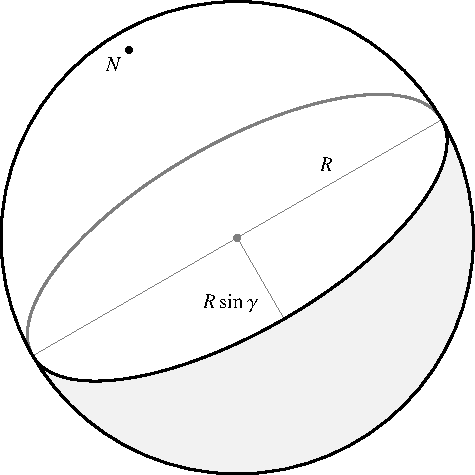
\includegraphics{chapters/5/halb.pdf}
\caption{Aufteilung der sonnenbeschienenen Seite der Erde durch den
Äquator.
\label{skript:halbkugel:teilung}}
\end{figure}%
Die einfachste Erweiterung des Modells von Budyko teilt die
Erde in zwei Halbkugeln auf, die Energie nur langsam austauschen
können.
Für die Energiebilanz brauchen wir daher die Strahlungsleistung
auf einer Halbkugel in Abhängigkeit von der Neigung $\gamma$ der
Erdachse.

Die gesamte auf auf die Erde eingestrahlte Leistung ist $\pi R^2S_0$.
Diese Leistung muss nun in Abhängigkeit von der Neigung $\gamma$
auf die beiden Halbkugeln verteilt werden.
Von der Erde aus gesehen teilt der Äquator die bestrahlte Erde wie
in Abbildung~\ref{skript:halbkugel:teilung} dargestellt.
Der Unterschied zwischen den beiden Halbkugeln ist der Flächeninhalt
der Ellipse, also
\[
F=\pi R^2\sin\gamma.
\]
Die Strahlungsleistung auf den beiden Halbkugeln in
Abbildung~\eqref{skript:halbkugel:teilung} ist daher
\begin{align}
E_N
&= 
\frac12(\pi R^2 S_0 +\pi R^2S_0\sin\gamma)
=
\pi R^2S_0 \frac{1+\sin\gamma}2 = Q\frac{1+\sin\gamma}2
&&\text{Nordhalbkugel,}
\\
E_S
&= 
\frac12(\pi R^2 S_0 -\pi R^2\sin\gamma)
=
\pi R^2S_0 \frac{1-\sin\gamma}2 = Q\frac{1-\sin\gamma}2
&&\text{Südhalbkugel.}
\end{align}
In Kapitel~\ref{chapter:neigung} wird diese Lösung verwendet, um zu
modellieren, wie die Veränderung der Neigung der Erdachse zu Eiszeiten
führen kann.





%
% einstrahlung.tex
%
% (c) 2018 Prof Dr Andreas Müller,Hochschule Rapperswil
%
\subsection{Einstrahlung auf einen Breitenkreis}
Wir berechnen die Einstrahlung auf einem gegebenen Breitengrad
$\vartheta$ in Abhängigkeit von der Neigung $\gamma$
der Erdachse.
Die einfallende Strahlungsleistung ist proportional zum Skalarprodukt
der Richtung der Einstrahlung mit der Normalen in einem Punkte
auf dem Breitenkreis zur Breite $\vartheta$.
Die Normale ist
\[
\vec n(\vartheta,\varphi)
=
\begin{pmatrix}
\sin\vartheta\cos\varphi\\
\sin\vartheta\sin\varphi\\
\cos\vartheta
\end{pmatrix}.
\]
Die Richtung der Einstrahlungsrichtung ist
\[
\vec e(\gamma)
=
\begin{pmatrix}
\cos\gamma\\
0\\
\sin\gamma
\end{pmatrix}.
\]
Das Skalarprodukt ist
\begin{equation}
\vec n(\vartheta,\varphi)\cdot\vec e(\gamma)
=
\sin\vartheta\cos\varphi\cos\gamma
+
\cos\vartheta\sin\gamma.
\label{skript:einstrahlung:skalarprodukt}
\end{equation}
Für die folgende Diskussion nehmen wir an, dass $\gamma >= 0$,
dass also der Nordpol permanent bestrahlt ist und der Südpol keine
Strahlung erhält.

Im Folgenden wollen wir die Energie berechnen, die in eine Zone
eingestrahlt wird.

\subsubsection{Sonnenauf- und -untergang}
Die Einstrahlung erfolgt natürlich nur zwischen Sonnenauf- und
-untergang.
Wir bezeichen die geographische Länge, bei der der Sonnenauf- oder
-untergang erfolgt, mit $\pm\varphi_0$.
Diese sind gekennzeichnet dadurch, dass $\vec n(\vartheta,\varphi_0)$ und
$\vec e(\gamma)$ senkrecht aufeinander stehen oder
\begin{equation*}
\begin{aligned}
&&
\vec n(\vartheta,\varphi_0)&\perp \vec e(\gamma)
\\
&\Rightarrow&
\vec n(\vartheta,\varphi_0)\cdot \vec e(\gamma)&=0
\\
&\Rightarrow&
\sin\vartheta\cos\varphi_0\cos\gamma
&=
-
\cos\vartheta\sin\gamma
\\
&\Rightarrow&
\cos\varphi_0
&=
-\frac{\tan\gamma}{\tan\vartheta}.
\end{aligned}
\end{equation*}
Wenn $\vartheta < \gamma$ (Punkt in der Nähe des Nordpols) oder
$\vartheta > \pi - \gamma$ (Punkt in der Nähe des Südpols),
dann hat die Gleichung keine Lösung,
die Sonne geht nie auf (Polarnacht) oder unter (Polartag).

\subsubsection{Mittlere Strahlungsleistung auf Breite $\vartheta$}
Um die Strahlungsleistung auf einer beliebigen geographischen
Breite zu berechnen, gehen wir in zwei Schritten vor.
Das Skalarprodukt~\eqref{skript:einstrahlung:skalarprodukt} 
gibt die Strahlungsleistung $\varepsilon(\vartheta,\varphi,\gamma)$
in einem Punkt auf der geographischen
Breite $\vartheta$ in Abhängigkeit von $\varphi$.
Im ersten Schritt mitteln wir dies über eine Umdrehung, dazu
ist das Skalarprodukt~\eqref{skript:einstrahlung:skalarprodukt} über eine
Umdrehung zu mitteln.
So erhalten wir die mittlere Strahlungsleistung $\varepsilon(\vartheta,\gamma)$
in einem Punkte auf geographischer Breite $\vartheta$.
Im zweiten Schritt müssen wir die die mittlere Strahlungsleistung mit
der Länge des Breitenkreises multiplizieren, um die Strahlungsleistung
auf dem Breitenkreis zur Breite $\vartheta$ zu erhalten.

\subsubsection{Polnähe}
In der Nähe des Südpols, also wenn $\vartheta > \pi - \gamma$,
ist die Einstrahlung $=0$.
In der Nähe des Nordpols, also wenn $\vartheta < \gamma$, ist die
Einstrahlungsdichte
\[
\varepsilon_{\text{in}}
=
\int_0^{2\pi}
\sin\vartheta\cos\varphi\cos\gamma
+
\cos\vartheta\sin\gamma
\,d\varphi
=
2\pi\cos\vartheta\sin\gamma.
\]
Für den Spezialfall $\vartheta=0$ fällt der erste Term weg und es
bleibt 
\begin{align*}
\varepsilon_{\text{in}}(0,\gamma)
&=
2\pi\sin\gamma.
\end{align*}

\subsubsection{Äquator}
Am Äquator ist $\vartheta=\frac{\pi}2$ und $\varphi_0=\frac{\pi}2$.
Man bekommt
\begin{align*}
\varepsilon_{\text{in}}\biggl(\frac{\pi}2,\gamma\biggr)
&=
\int_{-\varphi_0}^{\varphi_0}
\cos\varphi\cos\gamma\,d\varphi
=
\cos\gamma
\int_{-\frac{\pi}2}^{\frac{\pi}2}
\cos\varphi
\,d\varphi
=
2\cos\gamma
\end{align*}
für die Einstrahlung am Äquator.

\subsubsection{Der allgemeine Fall mit Sonnenauf- und -untergang}
\begin{figure}
\centering
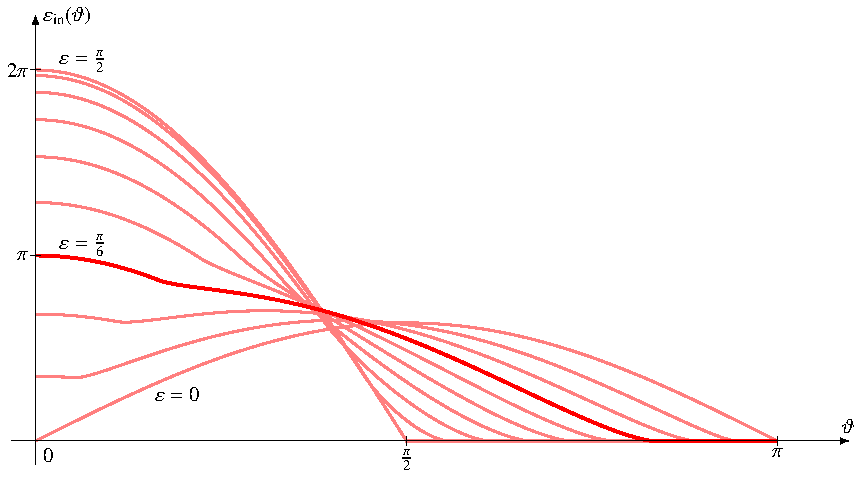
\includegraphics[width=\hsize]{chapters/5/ein.pdf}
\caption{Über eine Rotation gemittelte Einstrahlungsdichte
in Abhängigkeit von der geographischen Breite
gemäss Formel~\eqref{skript:einstrahlung:plottable} für verschiedene
Neigungen $\gamma$ der Achse. 
Dargestellt sind $\gamma$-Werte zwischen 0 und $90^\circ$ 
in $10^\circ$-Schritten. 
Die Neigung $\gamma=30^\circ=\frac{\pi}{6}$ ist hervorgehoben.
\label{skript:einstrahlung:ein}}
\end{figure}%
Der allgemeine Fall mit Sonnenauf- und -untergang
ist $\gamma < \vartheta < \pi-\gamma$.
Für die Einstrahlung finden wir dann
\begin{align}
\varepsilon_{\text{in}}(\vartheta,\gamma)
&=
\int_{-\varphi_0}^{\varphi_0}
\sin\vartheta\cos\varphi\cos\gamma
+
\cos\vartheta\sin\gamma\,d\varphi
\notag
\\
&=
\sin\vartheta\cos\gamma\biggl[\sin\varphi\biggr]_{-\varphi_0}^{\varphi_0}
+
2\varphi_0 \cos\vartheta\sin\gamma
\notag
\\
&=
2\sin\vartheta\cos\gamma\sin\varphi_0
+
2\varphi_0 \cos\vartheta\sin\gamma
\notag
\\
&=
2\sin\vartheta\cos\gamma
\sin
\arccos\biggl(-\frac{\tan\gamma}{\tan\vartheta}\biggr)
+
2\cos\vartheta\sin\gamma
\arccos\biggl(-\frac{\tan\gamma}{\tan\vartheta}\biggr).
\notag
\\
\intertext{Im ersten Term können wir $\sin\arccos x  = \sqrt{1-x^2}$
verwenden.
Den zweiten Term könnten wir so stehen lassen, aber für die graphische
Darstellung brauchen wir eine Darstellung das Arkuskosinus durch den
Arkustangens, da TikZ nur den Arkustangens anbietet.
Wir verwenden die Formel $\arccos x = 2\arctan\sqrt{(1-x)/(1+x)}$ und
erhalten}
&=
2\sin\vartheta\cos\gamma
\sqrt{1-\frac{\tan^2\gamma}{\tan^2\vartheta}}
+
4\cos\vartheta\sin\gamma
\arctan\sqrt{\frac{1+\frac{\tan\gamma}{\tan\vartheta}}{1-\frac{\tan\gamma}{\tan\vartheta}}}
\notag
\\
&=
\pm2\cos\vartheta\cos\gamma
\sqrt{\tan^2\vartheta-\tan^2\gamma}
+
4\cos\vartheta\sin\gamma
\arctan\sqrt{\frac{\tan\vartheta+\tan\gamma}{\tan\vartheta-\tan\gamma}}
\notag
\\
&=
2
\cos\vartheta
\biggl(
\cos\gamma
\sqrt{\frac{\tan^2\vartheta}{\tan^2\gamma}-1}
+
2
\sin\gamma
\arctan\sqrt{
\frac{\tan\vartheta+\tan\gamma}{\tan\vartheta-\tan\gamma}
}
\biggr).
\label{skript:einstrahlung:plottable}
\end{align}
Formel~\eqref{skript:einstrahlung:plottable} ist in
Abbildung~\ref{skript:einstrahlung:ein} dargestellt.

\subsubsection{Strahlungsleistung auf dem Breitenkreis $\vartheta$}
\begin{figure}
\centering
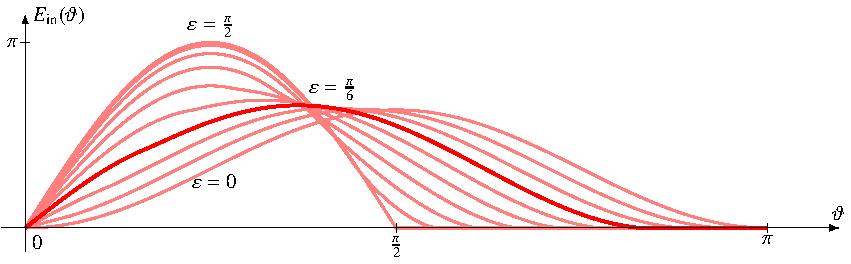
\includegraphics[width=\hsize]{chapters/5/ein1.pdf}
\caption{Strahlungsleistung auf geographischer Breite $\vartheta$,
gegeben durch Formel~\eqref{skript:einstrahlung:breite}.
\label{skript:einstrahlung:ein1}}
\end{figure}%
Die gesamte Strahlungsleistung auf dem Breitenkreis $\vartheta$
ist
\begin{equation}
E_{\text{in}}(\vartheta)
=
\varepsilon(\vartheta,\gamma)
\cdot
\sin\vartheta
\label{skript:einstrahlung:breite}
\end{equation}
Die resultierende Funktion ist in Abbildung~\ref{skript:einstrahlung:ein1}
dargestellt.

\subsection{Einstrahlung über ein Jahr}
\begin{figure}
\centering
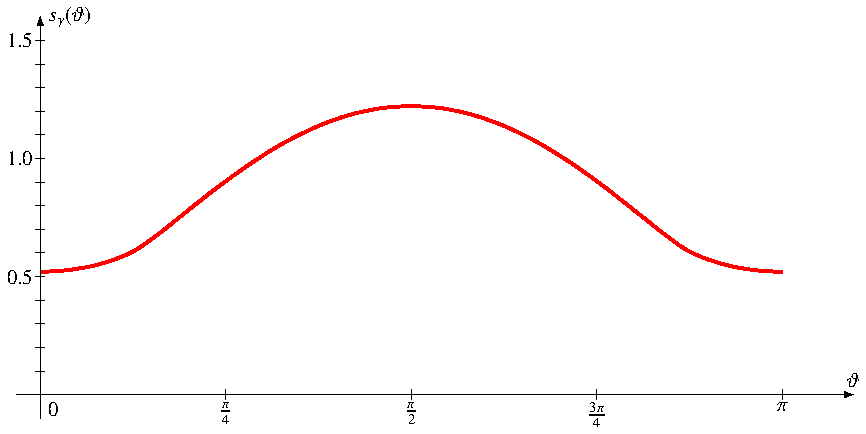
\includegraphics[width=\hsize]{chapters/5/total.pdf}
\caption{Einstrahlung über ein Jahr in Abhängigkeit von der geographischen
Breite.
\label{skript:einstrahlung:total}}
\end{figure}
Die in \eqref{skript:einstrahlung:breite} gefunden Einstrahlung auf einem
Breitengrad $\vartheta$ geht von einer konstanten Neigung der Erdachse aus.
Die Bewegung der Erde um die Sonne bedeutet aber, dass die Neigung der
der Erdachse scheinbar variert,
es gilt nämlich
\[
\tan \gamma(t) = \tan\gamma_\text{max}\cdot \sin t.
\]
Für ein Klimamodell wesentlich ist daher der Mittelwert
\[
s_{\gamma_\text{max}}(\vartheta)
=
\frac1{2\pi}
\int_0^{2\pi} \varepsilon(\vartheta,\gamma(t))\,dt
\]
von \eqref{skript:einstrahlung:breite} über ein Jahr.
Abbildung~\ref{skript:einstrahlung:total} zeigt das Resultat der 
numerischen Integration.










%
% bilanz.tex -- Bilanz-Modelle
%
% (c) 2018 Prof Dr Andreas Müller, Hochschule Rapperswil
%
\section{Strahlungsbilanzmodelle\label{skript:section:budyko}}
\rhead{Strahlunbsbilanzmodelle}
Im Kapitel~\ref{chapter:wetter und klima} haben wir die physikalischen
Grundlagen der Wetter und Klimaphänomene studiert.
In diesem Abschnitt wollen wir ein einfaches Modell für die Energiebilanz
der Erde entwickeln.

\subsection{Strahlungsbilanz\label{skript:subsection:strahlungsbilanz}}
Wir formulieren ein Modell mit einer einzigen Variablen, der globalen
Mitteltemperatur $T$.
Berechnet werden soll die zeitliche Entwicklung von $T$.

\subsubsection{Einstrahlung}
Die Erde mit Radius $R$ erhält ihre Energie von der Sonne, die
den konstanten Energiefluss $S_0 = 1368 \text{W\,m}^{-2}$
einstrahlt.
Der Querschnitt der Erde ist $\pi R^2$, auf den eine Leistung von
$\pi R^2 S_0$ fällt.
Die Atmosphäre und die Weltmeere transportieren diese Energie, wir nehmen
an, sie gleichmässig über die ganze Erdoberfläche verteilt wird.
Die pro Flächeneinheit anfallende Leistung ist daher
\begin{equation}
\frac{\pi R^2 S_0}{4\pi R^2} = \frac14S_0=Q.
\label{skript:bilanz:einstrahlung}
\end{equation}

Doch kann nicht die gesamte Energie absorbiert werden.
Ein Teil wird von Wolken oder von Eis an der Oberfläche 
gleich wieder reflektiert, aber auch Landmassen und die Meere reflektieren
einen kleineren Teil der Strahlung.
Die auf Seite~\pageref{skript:subsubsection:albedo} beschriebene Albedo
hat für die Erde Werte zwischen $0.3$ und $0.7$ je nach dem Grad der
Bewölkung und der Vereisung.
Bei tieferer Temperatur muss mit stärkerer Vereisung und mehr Wolken
gerechnet werden.
Sei $\alpha(T)$ die Albedo der Erde bei der Temperatur $T$.
Der von der Erde absorbierte Fluss ist daher
\begin{equation}
(1-\alpha(T)) Q.
\label{skript:bilanz:ausstrahlung}
\end{equation}
Die Grösse $1-\alpha(T)$ heisst auch die {\em Coalbedo}.
\index{Coalbedo}%

\subsubsection{Ausstrahlung}
Die Erde verliert Energie auch wieder durch Strahlung.
Nach dem Stefan-Boltzmannschen Gesetz~\eqref{skript:stefon-boltzmann}
ist die Ausstrahlung der Erde proportional zur vierten Potenz der
Temperatur, also $T^4$.

\subsubsection{Bilanzgleichung}
Die Temperatur ändert sich umso mehr, je grösser das Ungleichgewicht
zwischen Einstrahlung \eqref{skript:bilanz:einstrahlung} und
\eqref{skript:bilanz:ausstrahlung} ist.
Die Wärmekapazität der Erdoberfläche spielt ebenfalls
eine Rolle, je grösser diese ist, desto träger folgt die Temperatur dem
Energiebilanzüberschuss.

Wir erhalten so die Differentialgleichung
\begin{equation}
C\frac{dT}{dt}
=
(1-\alpha(T)) Q - \sigma T^4.
\label{skript:bilanz:basic}
\end{equation}
Je grösser $C$ ist, desto kleiner ist die Änderungsgeschwindigkeit der
globalen Mitteltemperatur bei gleicher rechter Seite.

\subsubsection{Gleichgewichtslösung}
Wir suchen eine Gleichgewichtslösung für dieses Modell, und nehmen zu diesem
Zweck den typischen Wert $\alpha=0.3$ der Albedo der Erde.
Sie muss $\dot T=0$ erfüllen, also
\begin{align*}
(1-\alpha) Q -\sigma T^4 &=0
\\
\Rightarrow
\qquad
T&=\root 4\of{\frac{(1-\alpha)Q}{\sigma}}
\end{align*}
Setzt man die üblichen Werte für $Q$ ein, erhält man eine globale
Mitteltemperatur von $T=254.8\,\text{K}$.

\subsubsection{Treibhauseffekt}
Die tatsächliche global Mitteltemperatur $T=287.7\,\text{K}$ ist.
Diese Diskrepanz ist zwei Unzulänglichkeiten diesen einfachen
Modells zurückzuführen:
\begin{enumerate}
\item
Der Treibhauseffekt sorgt dafür, dass nur ein Teil der abgestrahlten
Wärmestrahlung die Erde tatsächlich verlässt.
Wir können dies dadurch modellieren, dass wir in der Gleichung
\eqref{skript:bilanz:basic} den Ausstrahlungsterm um einen Faktor
$\varepsilon$ reduzieren, der den Treibhauseffekt modellieren soll.
Die neue Grundgleichung wird dann
\begin{equation}
C\frac{dT}{dt}
=
(1-\alpha(T)) Q - \varepsilon\sigma T^4.
\label{skript:bilanz:basic2}
\end{equation}
Um die aktuelle Gleichgewichtstemperatur $T=287.7\,\text{K}$ von 2010
zu reproduzieren müssen wir $\varepsilon=0.32$ wählen.
\item
Die Albedo hängt von der Temperatur ab und wird mit abnehmender 
Temperatur grösser.
Bei sehr tiefen Temperaturen kann die Albedo auf bis $0.7$ steigen.
Ein einfaches Modell, welches Diesen Sachverhalt abbildet, ist
\begin{equation}
\alpha(T)=0.5-0.2\tanh\biggl(\frac{T-265}{10}\biggr)
\label{skript:bilanz:albedo}
\end{equation}
\end{enumerate}

\subsubsection{Gleichgewichte}
\begin{figure}
\centering
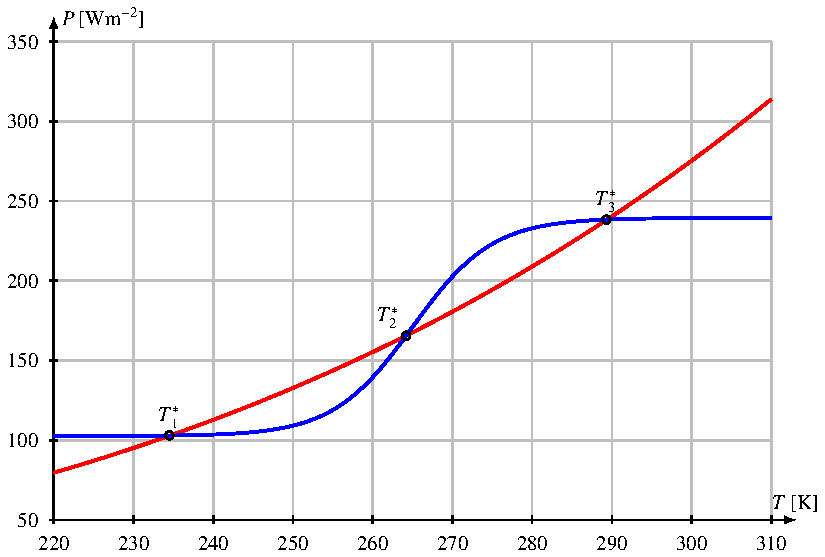
\includegraphics{chapters/5/bilanzmodell.pdf}
\caption{Einstrahlung und Ausstrahlung in dem einfachen Bilanzmodell
mit der Modellgleichung
\eqref{skript:bilanz:basic2} und der Albedo-Funktion
\eqref{skript:bilanz:albedo}.
Die Ausstrahlung $\varepsilon\sigma T^4$ ist rot eingezeichnet,
blau ist die Ausstrahlung.
Es entstehen drei Gleichgewichtspunkte $T_1^*$, $T_2^2*$ und $T_3^*$,
von denen aber $T_2^*$ nicht stabil ist.
\label{skript:bilanz:modellbild}}
\end{figure}
Das Modell mit der Albedo-Funktion~\eqref{skript:bilanz:albedo}
hat nicht nur einen sondern drei Gleichgewichtspunkte.
Die Einstrahlung und die Ausstrahlung ist in
Abbildung~\ref{skript:bilanz:modellbild} dargestellt.

Die beiden Gleichgewichtspunkte $T_1^*$ und $T_3^*$ sind stabil.
In beiden Punkten ändert sich die absorbierte Energie kaum bei
einer Temperaturänderung, aber die Ausstrahlung wird bei erhöhter 
Temperatur wesentlich effizienter, so dass sich die Erde wieder
abkühlt.
Ebenso verringert sich die Ausstrahlung bei leicht tieferer Temperatur
sofort, so dass die Erde sich wieder zur Gleichgewichtstemperatur aufwärmen
kann.

Das Gleichgewicht $T_2^*$ ist dagegen nicht stabil.
Bei höherer Temperatur wird die Einstrahlung sofort grösser, ohne dass
die Ausstrahlung mithalten kann, so dass sich die Erde weiter
aufwärmt bis zur Temperatur $T_3^*$.
Bei leicht tieferer Temperatur steigt die Albedo stark an so dass die
Einstrahlung schnell abnimmt, während die Ausstrahlung nur vergleichsweise
langsam zurückgeht, die Erde kühlt sich bis auf die Temperatur $T_1^*$ ab.

\subsubsection{Bifurkation und globale Erwärmung}
\begin{figure}
\centering
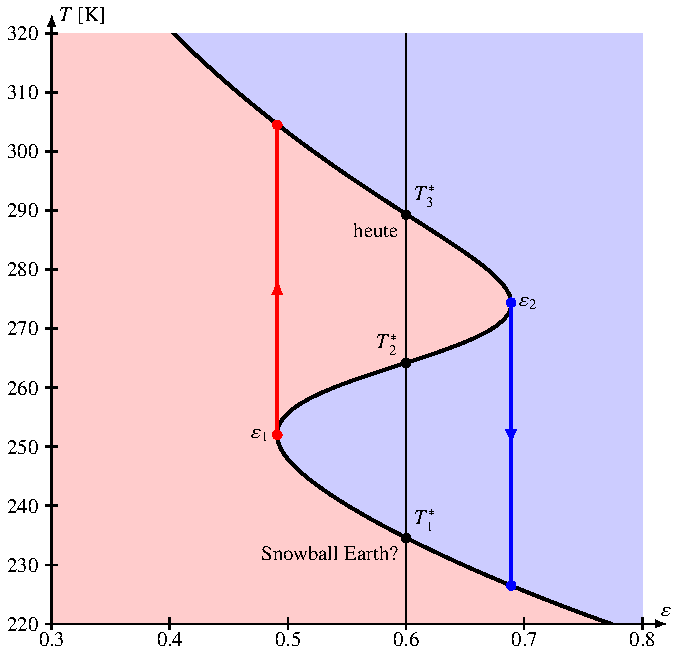
\includegraphics{chapters/5/bifurkation.pdf}
\caption{Bifurkationsdiagramm für das Bilanzmodell
\eqref{skript:bilanz:basic2}
in Abhängigkeit vom Treibhauseffekt-Parameter $\varepsilon$.
\label{skript:bilanz:bifurkation}}
\end{figure}
Der Parameter $\varepsilon$ modelliert den Treibhauseffekt.
Steigt die Konzentration der Klimagase in der Atmosphäre, wird die
abgestrahlten Leistung geringer, also $\varepsilon$ kleiner.
Es lohnt sich daher, die Entwicklung des Gleichgewichtspunkte in 
Abhängigkeit von $\varepsilon$ zu untersuchen.
Das Bifurkationsdiagramm des Modells
\eqref{skript:bilanz:basic2} in Abhängigkeit von $\varepsilon$
ist in Abbildung~\ref{skript:bilanz:bifurkation} dargestellt.

Man kann aus dem Diagramm ablesen, dass mit weitterer Zunahme des 
Treibhauseffektes, als mit Abnahme von $\varepsilon$, die globale
Mitteltemperatur weiter ansteigen wird.
Sinkt $\varepsilon$ unter den kritischen Wert $\varepsilon_1$ steigt die
Temperatur auf über $305\,\text{K}$.
In diesem Fall verschwinden die beiden Gleichgewichtspunkte $T_1^*$
und $T_2^*$, es bleibt nur das Gleichgewicht $T_3^*$.

Interessant ist aber auch, was bei starker Abnahme der
Treibhausgaskonzentration passiert.
Wenn $\varepsilon$ über $\varepsilon_2$ ansteigt, dann verschwinde
$T_3^*$ und $T_2^*$, es bleibt nur der Gleichgewichtspunkt $T_1^*$,
bei dem die ganze auf sehr tiefer Temperatur vereist.
Man vermutet, dass genau dieser Zustand in der Phase des {\em Snowball Earth}
eingetreten ist, als die ersten photosynthetisierenden Organismen die
Treibhausgase dramatische reduziert und damit $\varepsilon$ stark
erhöht hatten.
Man beachte dass es nur möglich ist, den heutigen Zustand wieder zu 
erreichen, indem die Treibhausgaskonzentration soweit gesteigert
wird, dass $\varepsilon<\varepsilon_1$ wird.
Es muss im Laufe der Erdgeschichte also nach der Snowball Earth Phase
auch Phasen mit wesentlich höherer Treibhausgaskonzentration als heute
gegeben haben.

\subsection{Modell von Budyko\label{subsection:modell von budyko}}
Bisher haben wir die Ausstrahlung mit Hilfe des Stefan-Boltzmannschen
Gesetzes für die Strahlung eines schwarzen Körpers modelliert.
Es ist fraglich, ob dies tatsächlich zutreffend ist.
Die Ausstrahlung $E_\text{out}(T)$ der Ausstrahlung könnte also durchaus
eine kompliziertere Funktion sein.
Sie muss aber so beschaffen sein, dass sich bei der aktuellen
Mitteltemperatur $T^*$ ein stabiles Gleichgewicht ergibt.
In der Umgebung des Gleichgewichtes kann die Funktion $E_\text{out}(T)$
als lineare Funktion
$E_\text{out}= A+BT$
dargestellt werden.
Nahe bei $T^*$ kann die globale Mitteltemperatur also mit einem Modell
der Form
\begin{equation}
C
\frac{dT}{dt}
=
(1-\alpha(T)) Q- (A+BT)
\end{equation}
beschrieben werden.
Das Gleichgewicht erfüllt
\[
(1-\alpha(T^*))Q=A+BT^*
\] 
und ist stabil, wenn die Steigung der Einstrahlung kleiner ist als die
Die Steigung der Ausstrahlung, also
\begin{equation}
-Q\alpha'(T)
<
B.
\label{skript:budyko:cond}
\end{equation}
Dieses Modell wurde schon in den sechziger Jahren von Budyko vorgeschlagen.
Zahlenwerte für $A$ und $B$ konnte seit der damaligen Zeit durch
Satellitenmessungen bestimmt werden.

Die Folgen des Treibhauseffektes sind auch in diesem einfacheren Modell
nachvollziehbar.
Die Erhöhung der Treibhausgaskonzentration reduziert die Ausstrahlung,
was sich zum Beispiel in einem kleineren Wert von $B$ äussert.
Eine Abnahme von $B$ um $\Delta B$ führt zu einer
Änderung der Gleichgewichtstemperatur um $\Delta T$, die die Gleichung
\begin{align*}
(1-\alpha(T^*+\Delta T))Q
&=
A + (B-\Delta B)(T^*+\Delta T)
\\
\underbrace{(1-\alpha(T^*))Q}_{\displaystyle=A+BT^*}
-Q\alpha'(T^*)\Delta T
&=
A+BT^*
- T^*\Delta B
+B\Delta T
\\
(Q\alpha'(T^*)
+
B)\Delta T
&=
T^*
\Delta B
\\
\Delta T
&=
\frac{T^*\Delta B}{Q\alpha'(T^*)+B}
\end{align*}
erfüllt.
Man kann daraus ablesen, dass eine Abnahme von $B$ genau dann zu einer
Zunahme der Mitteltemperatur, wenn der Nenner positiv ist, also
\[
Q\alpha'(T^*)+B > 0
\qquad\Rightarrow\qquad
-Q\alpha'(T^*)<B,
\]
was die Bedingung
\eqref{skript:budyko:cond}
beweist.





%
% zonen.tex -- Zonenmodelle für das Klima
%
% (c) 2018 Prof Dr Andreas Müller, Hochschule Rapperswil
%
\chapter{Zonenmodelle\label{chapter:zonenmodelle}}
\lhead{Kapitel \thechapter: Zonenmodelle}
Die Erdrotation ist schnell im Vergleich zu den für typische Klimamodelle
wesentlichen Zeitspannen.
Wesentliche Aspekte der Klimaentwicklung sollten sich daher immer
noch modellieren lassen, wenn man den Zustand des Klimasystems über
die Erdrotation mittelt.
In diesem Kapitel werden daher vereinfachte Modelle diskutiert,
die nur die geographischen Länge als geometrischen Parameter haben.

%
% strahlung.tex
%
% (c) 2018 Prof Dr Andreas Müller, Hochschule Rapperswil
%
\section{Strahlung\label{section:strahlung}}
\rhead{Strahlung}
Die von der Erde empfange Strahlung sowie die Albedo wurden bereits in
Abschnitt~\ref{skript:grundlagen:strahlung} untersucht.
Für die später in diesem Kapitel zu untersuchenden Modelle ist aber
erforderlich, die örtliche Verteilung der Strahlung auf der Erdoberfläche
genauer zu verstehen.
In diesem Abschnitt wird daher zuerst die Strahlungsleistung auf einer
Halbkugel und später auf einer Zone um einen Breitenkreis berechnet.
%
% halbkugel.tex -- Einstrahlung auf eine Halbkugel
%
% (c) 2018 Prof Dr Andreas Müller, Hochschule Rapperswil
%
\subsection{Einstrahlung auf einer Halbkugel\label{subsection:halbkugel}}
\begin{figure}
\centering
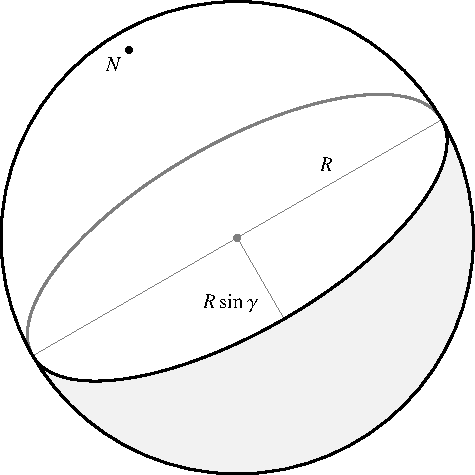
\includegraphics{chapters/5/halb.pdf}
\caption{Aufteilung der sonnenbeschienenen Seite der Erde durch den
Äquator.
\label{skript:halbkugel:teilung}}
\end{figure}%
Die einfachste Erweiterung des Modells von Budyko teilt die
Erde in zwei Halbkugeln auf, die Energie nur langsam austauschen
können.
Für die Energiebilanz brauchen wir daher die Strahlungsleistung
auf einer Halbkugel in Abhängigkeit von der Neigung $\gamma$ der
Erdachse.

Die gesamte auf auf die Erde eingestrahlte Leistung ist $\pi R^2S_0$.
Diese Leistung muss nun in Abhängigkeit von der Neigung $\gamma$
auf die beiden Halbkugeln verteilt werden.
Von der Erde aus gesehen teilt der Äquator die bestrahlte Erde wie
in Abbildung~\ref{skript:halbkugel:teilung} dargestellt.
Der Unterschied zwischen den beiden Halbkugeln ist der Flächeninhalt
der Ellipse, also
\[
F=\pi R^2\sin\gamma.
\]
Die Strahlungsleistung auf den beiden Halbkugeln in
Abbildung~\eqref{skript:halbkugel:teilung} ist daher
\begin{align}
E_N
&= 
\frac12(\pi R^2 S_0 +\pi R^2S_0\sin\gamma)
=
\pi R^2S_0 \frac{1+\sin\gamma}2 = Q\frac{1+\sin\gamma}2
&&\text{Nordhalbkugel,}
\\
E_S
&= 
\frac12(\pi R^2 S_0 -\pi R^2\sin\gamma)
=
\pi R^2S_0 \frac{1-\sin\gamma}2 = Q\frac{1-\sin\gamma}2
&&\text{Südhalbkugel.}
\end{align}
In Kapitel~\ref{chapter:neigung} wird diese Lösung verwendet, um zu
modellieren, wie die Veränderung der Neigung der Erdachse zu Eiszeiten
führen kann.





%
% einstrahlung.tex
%
% (c) 2018 Prof Dr Andreas Müller,Hochschule Rapperswil
%
\subsection{Einstrahlung auf einen Breitenkreis}
Wir berechnen die Einstrahlung auf einem gegebenen Breitengrad
$\vartheta$ in Abhängigkeit von der Neigung $\gamma$
der Erdachse.
Die einfallende Strahlungsleistung ist proportional zum Skalarprodukt
der Richtung der Einstrahlung mit der Normalen in einem Punkte
auf dem Breitenkreis zur Breite $\vartheta$.
Die Normale ist
\[
\vec n(\vartheta,\varphi)
=
\begin{pmatrix}
\sin\vartheta\cos\varphi\\
\sin\vartheta\sin\varphi\\
\cos\vartheta
\end{pmatrix}.
\]
Die Richtung der Einstrahlungsrichtung ist
\[
\vec e(\gamma)
=
\begin{pmatrix}
\cos\gamma\\
0\\
\sin\gamma
\end{pmatrix}.
\]
Das Skalarprodukt ist
\begin{equation}
\vec n(\vartheta,\varphi)\cdot\vec e(\gamma)
=
\sin\vartheta\cos\varphi\cos\gamma
+
\cos\vartheta\sin\gamma.
\label{skript:einstrahlung:skalarprodukt}
\end{equation}
Für die folgende Diskussion nehmen wir an, dass $\gamma >= 0$,
dass also der Nordpol permanent bestrahlt ist und der Südpol keine
Strahlung erhält.

Im Folgenden wollen wir die Energie berechnen, die in eine Zone
eingestrahlt wird.

\subsubsection{Sonnenauf- und -untergang}
Die Einstrahlung erfolgt natürlich nur zwischen Sonnenauf- und
-untergang.
Wir bezeichen die geographische Länge, bei der der Sonnenauf- oder
-untergang erfolgt, mit $\pm\varphi_0$.
Diese sind gekennzeichnet dadurch, dass $\vec n(\vartheta,\varphi_0)$ und
$\vec e(\gamma)$ senkrecht aufeinander stehen oder
\begin{equation*}
\begin{aligned}
&&
\vec n(\vartheta,\varphi_0)&\perp \vec e(\gamma)
\\
&\Rightarrow&
\vec n(\vartheta,\varphi_0)\cdot \vec e(\gamma)&=0
\\
&\Rightarrow&
\sin\vartheta\cos\varphi_0\cos\gamma
&=
-
\cos\vartheta\sin\gamma
\\
&\Rightarrow&
\cos\varphi_0
&=
-\frac{\tan\gamma}{\tan\vartheta}.
\end{aligned}
\end{equation*}
Wenn $\vartheta < \gamma$ (Punkt in der Nähe des Nordpols) oder
$\vartheta > \pi - \gamma$ (Punkt in der Nähe des Südpols),
dann hat die Gleichung keine Lösung,
die Sonne geht nie auf (Polarnacht) oder unter (Polartag).

\subsubsection{Mittlere Strahlungsleistung auf Breite $\vartheta$}
Um die Strahlungsleistung auf einer beliebigen geographischen
Breite zu berechnen, gehen wir in zwei Schritten vor.
Das Skalarprodukt~\eqref{skript:einstrahlung:skalarprodukt} 
gibt die Strahlungsleistung $\varepsilon(\vartheta,\varphi,\gamma)$
in einem Punkt auf der geographischen
Breite $\vartheta$ in Abhängigkeit von $\varphi$.
Im ersten Schritt mitteln wir dies über eine Umdrehung, dazu
ist das Skalarprodukt~\eqref{skript:einstrahlung:skalarprodukt} über eine
Umdrehung zu mitteln.
So erhalten wir die mittlere Strahlungsleistung $\varepsilon(\vartheta,\gamma)$
in einem Punkte auf geographischer Breite $\vartheta$.
Im zweiten Schritt müssen wir die die mittlere Strahlungsleistung mit
der Länge des Breitenkreises multiplizieren, um die Strahlungsleistung
auf dem Breitenkreis zur Breite $\vartheta$ zu erhalten.

\subsubsection{Polnähe}
In der Nähe des Südpols, also wenn $\vartheta > \pi - \gamma$,
ist die Einstrahlung $=0$.
In der Nähe des Nordpols, also wenn $\vartheta < \gamma$, ist die
Einstrahlungsdichte
\[
\varepsilon_{\text{in}}
=
\int_0^{2\pi}
\sin\vartheta\cos\varphi\cos\gamma
+
\cos\vartheta\sin\gamma
\,d\varphi
=
2\pi\cos\vartheta\sin\gamma.
\]
Für den Spezialfall $\vartheta=0$ fällt der erste Term weg und es
bleibt 
\begin{align*}
\varepsilon_{\text{in}}(0,\gamma)
&=
2\pi\sin\gamma.
\end{align*}

\subsubsection{Äquator}
Am Äquator ist $\vartheta=\frac{\pi}2$ und $\varphi_0=\frac{\pi}2$.
Man bekommt
\begin{align*}
\varepsilon_{\text{in}}\biggl(\frac{\pi}2,\gamma\biggr)
&=
\int_{-\varphi_0}^{\varphi_0}
\cos\varphi\cos\gamma\,d\varphi
=
\cos\gamma
\int_{-\frac{\pi}2}^{\frac{\pi}2}
\cos\varphi
\,d\varphi
=
2\cos\gamma
\end{align*}
für die Einstrahlung am Äquator.

\subsubsection{Der allgemeine Fall mit Sonnenauf- und -untergang}
\begin{figure}
\centering
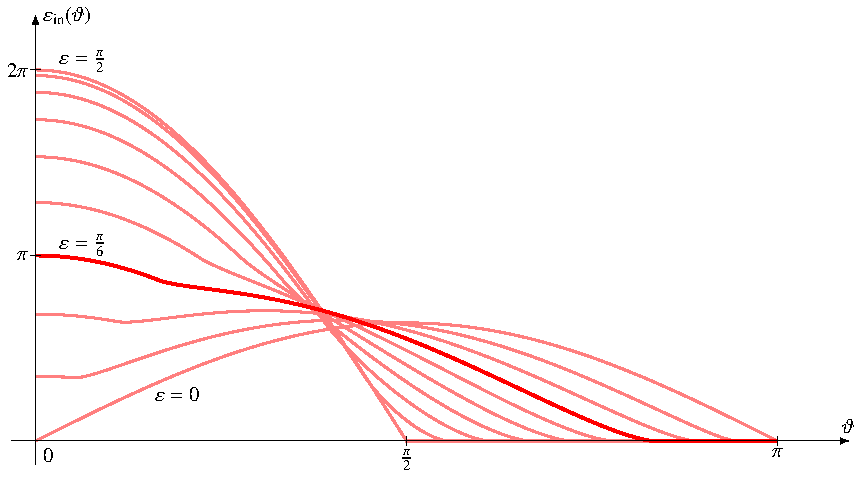
\includegraphics[width=\hsize]{chapters/5/ein.pdf}
\caption{Über eine Rotation gemittelte Einstrahlungsdichte
in Abhängigkeit von der geographischen Breite
gemäss Formel~\eqref{skript:einstrahlung:plottable} für verschiedene
Neigungen $\gamma$ der Achse. 
Dargestellt sind $\gamma$-Werte zwischen 0 und $90^\circ$ 
in $10^\circ$-Schritten. 
Die Neigung $\gamma=30^\circ=\frac{\pi}{6}$ ist hervorgehoben.
\label{skript:einstrahlung:ein}}
\end{figure}%
Der allgemeine Fall mit Sonnenauf- und -untergang
ist $\gamma < \vartheta < \pi-\gamma$.
Für die Einstrahlung finden wir dann
\begin{align}
\varepsilon_{\text{in}}(\vartheta,\gamma)
&=
\int_{-\varphi_0}^{\varphi_0}
\sin\vartheta\cos\varphi\cos\gamma
+
\cos\vartheta\sin\gamma\,d\varphi
\notag
\\
&=
\sin\vartheta\cos\gamma\biggl[\sin\varphi\biggr]_{-\varphi_0}^{\varphi_0}
+
2\varphi_0 \cos\vartheta\sin\gamma
\notag
\\
&=
2\sin\vartheta\cos\gamma\sin\varphi_0
+
2\varphi_0 \cos\vartheta\sin\gamma
\notag
\\
&=
2\sin\vartheta\cos\gamma
\sin
\arccos\biggl(-\frac{\tan\gamma}{\tan\vartheta}\biggr)
+
2\cos\vartheta\sin\gamma
\arccos\biggl(-\frac{\tan\gamma}{\tan\vartheta}\biggr).
\notag
\\
\intertext{Im ersten Term können wir $\sin\arccos x  = \sqrt{1-x^2}$
verwenden.
Den zweiten Term könnten wir so stehen lassen, aber für die graphische
Darstellung brauchen wir eine Darstellung das Arkuskosinus durch den
Arkustangens, da TikZ nur den Arkustangens anbietet.
Wir verwenden die Formel $\arccos x = 2\arctan\sqrt{(1-x)/(1+x)}$ und
erhalten}
&=
2\sin\vartheta\cos\gamma
\sqrt{1-\frac{\tan^2\gamma}{\tan^2\vartheta}}
+
4\cos\vartheta\sin\gamma
\arctan\sqrt{\frac{1+\frac{\tan\gamma}{\tan\vartheta}}{1-\frac{\tan\gamma}{\tan\vartheta}}}
\notag
\\
&=
\pm2\cos\vartheta\cos\gamma
\sqrt{\tan^2\vartheta-\tan^2\gamma}
+
4\cos\vartheta\sin\gamma
\arctan\sqrt{\frac{\tan\vartheta+\tan\gamma}{\tan\vartheta-\tan\gamma}}
\notag
\\
&=
2
\cos\vartheta
\biggl(
\cos\gamma
\sqrt{\frac{\tan^2\vartheta}{\tan^2\gamma}-1}
+
2
\sin\gamma
\arctan\sqrt{
\frac{\tan\vartheta+\tan\gamma}{\tan\vartheta-\tan\gamma}
}
\biggr).
\label{skript:einstrahlung:plottable}
\end{align}
Formel~\eqref{skript:einstrahlung:plottable} ist in
Abbildung~\ref{skript:einstrahlung:ein} dargestellt.

\subsubsection{Strahlungsleistung auf dem Breitenkreis $\vartheta$}
\begin{figure}
\centering
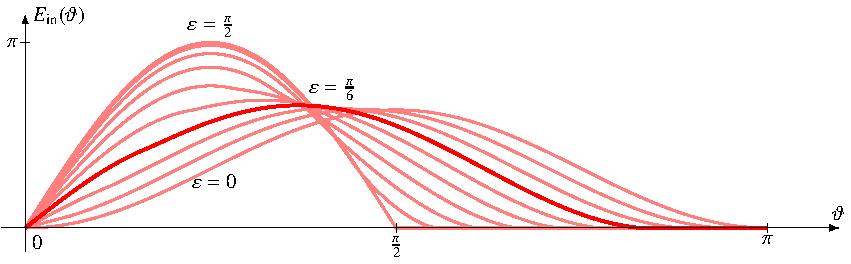
\includegraphics[width=\hsize]{chapters/5/ein1.pdf}
\caption{Strahlungsleistung auf geographischer Breite $\vartheta$,
gegeben durch Formel~\eqref{skript:einstrahlung:breite}.
\label{skript:einstrahlung:ein1}}
\end{figure}%
Die gesamte Strahlungsleistung auf dem Breitenkreis $\vartheta$
ist
\begin{equation}
E_{\text{in}}(\vartheta)
=
\varepsilon(\vartheta,\gamma)
\cdot
\sin\vartheta
\label{skript:einstrahlung:breite}
\end{equation}
Die resultierende Funktion ist in Abbildung~\ref{skript:einstrahlung:ein1}
dargestellt.

\subsection{Einstrahlung über ein Jahr}
\begin{figure}
\centering
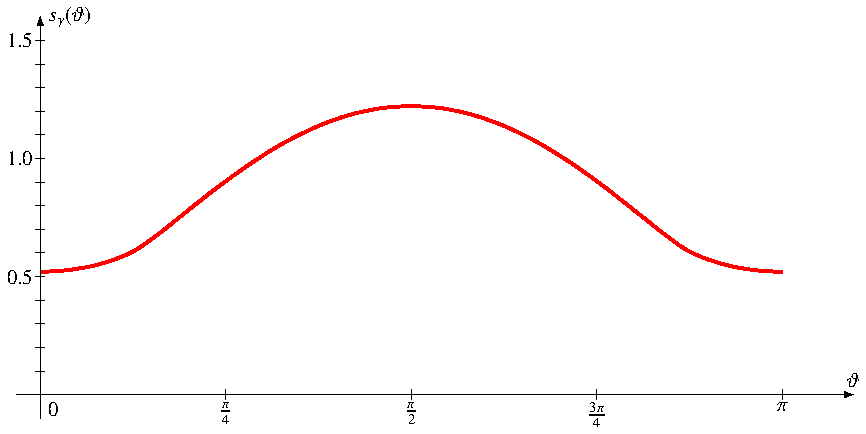
\includegraphics[width=\hsize]{chapters/5/total.pdf}
\caption{Einstrahlung über ein Jahr in Abhängigkeit von der geographischen
Breite.
\label{skript:einstrahlung:total}}
\end{figure}
Die in \eqref{skript:einstrahlung:breite} gefunden Einstrahlung auf einem
Breitengrad $\vartheta$ geht von einer konstanten Neigung der Erdachse aus.
Die Bewegung der Erde um die Sonne bedeutet aber, dass die Neigung der
der Erdachse scheinbar variert,
es gilt nämlich
\[
\tan \gamma(t) = \tan\gamma_\text{max}\cdot \sin t.
\]
Für ein Klimamodell wesentlich ist daher der Mittelwert
\[
s_{\gamma_\text{max}}(\vartheta)
=
\frac1{2\pi}
\int_0^{2\pi} \varepsilon(\vartheta,\gamma(t))\,dt
\]
von \eqref{skript:einstrahlung:breite} über ein Jahr.
Abbildung~\ref{skript:einstrahlung:total} zeigt das Resultat der 
numerischen Integration.










%
% bilanz.tex -- Bilanz-Modelle
%
% (c) 2018 Prof Dr Andreas Müller, Hochschule Rapperswil
%
\section{Strahlungsbilanzmodelle\label{skript:section:budyko}}
\rhead{Strahlunbsbilanzmodelle}
Im Kapitel~\ref{chapter:wetter und klima} haben wir die physikalischen
Grundlagen der Wetter und Klimaphänomene studiert.
In diesem Abschnitt wollen wir ein einfaches Modell für die Energiebilanz
der Erde entwickeln.

\subsection{Strahlungsbilanz\label{skript:subsection:strahlungsbilanz}}
Wir formulieren ein Modell mit einer einzigen Variablen, der globalen
Mitteltemperatur $T$.
Berechnet werden soll die zeitliche Entwicklung von $T$.

\subsubsection{Einstrahlung}
Die Erde mit Radius $R$ erhält ihre Energie von der Sonne, die
den konstanten Energiefluss $S_0 = 1368 \text{W\,m}^{-2}$
einstrahlt.
Der Querschnitt der Erde ist $\pi R^2$, auf den eine Leistung von
$\pi R^2 S_0$ fällt.
Die Atmosphäre und die Weltmeere transportieren diese Energie, wir nehmen
an, sie gleichmässig über die ganze Erdoberfläche verteilt wird.
Die pro Flächeneinheit anfallende Leistung ist daher
\begin{equation}
\frac{\pi R^2 S_0}{4\pi R^2} = \frac14S_0=Q.
\label{skript:bilanz:einstrahlung}
\end{equation}

Doch kann nicht die gesamte Energie absorbiert werden.
Ein Teil wird von Wolken oder von Eis an der Oberfläche 
gleich wieder reflektiert, aber auch Landmassen und die Meere reflektieren
einen kleineren Teil der Strahlung.
Die auf Seite~\pageref{skript:subsubsection:albedo} beschriebene Albedo
hat für die Erde Werte zwischen $0.3$ und $0.7$ je nach dem Grad der
Bewölkung und der Vereisung.
Bei tieferer Temperatur muss mit stärkerer Vereisung und mehr Wolken
gerechnet werden.
Sei $\alpha(T)$ die Albedo der Erde bei der Temperatur $T$.
Der von der Erde absorbierte Fluss ist daher
\begin{equation}
(1-\alpha(T)) Q.
\label{skript:bilanz:ausstrahlung}
\end{equation}
Die Grösse $1-\alpha(T)$ heisst auch die {\em Coalbedo}.
\index{Coalbedo}%

\subsubsection{Ausstrahlung}
Die Erde verliert Energie auch wieder durch Strahlung.
Nach dem Stefan-Boltzmannschen Gesetz~\eqref{skript:stefon-boltzmann}
ist die Ausstrahlung der Erde proportional zur vierten Potenz der
Temperatur, also $T^4$.

\subsubsection{Bilanzgleichung}
Die Temperatur ändert sich umso mehr, je grösser das Ungleichgewicht
zwischen Einstrahlung \eqref{skript:bilanz:einstrahlung} und
\eqref{skript:bilanz:ausstrahlung} ist.
Die Wärmekapazität der Erdoberfläche spielt ebenfalls
eine Rolle, je grösser diese ist, desto träger folgt die Temperatur dem
Energiebilanzüberschuss.

Wir erhalten so die Differentialgleichung
\begin{equation}
C\frac{dT}{dt}
=
(1-\alpha(T)) Q - \sigma T^4.
\label{skript:bilanz:basic}
\end{equation}
Je grösser $C$ ist, desto kleiner ist die Änderungsgeschwindigkeit der
globalen Mitteltemperatur bei gleicher rechter Seite.

\subsubsection{Gleichgewichtslösung}
Wir suchen eine Gleichgewichtslösung für dieses Modell, und nehmen zu diesem
Zweck den typischen Wert $\alpha=0.3$ der Albedo der Erde.
Sie muss $\dot T=0$ erfüllen, also
\begin{align*}
(1-\alpha) Q -\sigma T^4 &=0
\\
\Rightarrow
\qquad
T&=\root 4\of{\frac{(1-\alpha)Q}{\sigma}}
\end{align*}
Setzt man die üblichen Werte für $Q$ ein, erhält man eine globale
Mitteltemperatur von $T=254.8\,\text{K}$.

\subsubsection{Treibhauseffekt}
Die tatsächliche global Mitteltemperatur $T=287.7\,\text{K}$ ist.
Diese Diskrepanz ist zwei Unzulänglichkeiten diesen einfachen
Modells zurückzuführen:
\begin{enumerate}
\item
Der Treibhauseffekt sorgt dafür, dass nur ein Teil der abgestrahlten
Wärmestrahlung die Erde tatsächlich verlässt.
Wir können dies dadurch modellieren, dass wir in der Gleichung
\eqref{skript:bilanz:basic} den Ausstrahlungsterm um einen Faktor
$\varepsilon$ reduzieren, der den Treibhauseffekt modellieren soll.
Die neue Grundgleichung wird dann
\begin{equation}
C\frac{dT}{dt}
=
(1-\alpha(T)) Q - \varepsilon\sigma T^4.
\label{skript:bilanz:basic2}
\end{equation}
Um die aktuelle Gleichgewichtstemperatur $T=287.7\,\text{K}$ von 2010
zu reproduzieren müssen wir $\varepsilon=0.32$ wählen.
\item
Die Albedo hängt von der Temperatur ab und wird mit abnehmender 
Temperatur grösser.
Bei sehr tiefen Temperaturen kann die Albedo auf bis $0.7$ steigen.
Ein einfaches Modell, welches Diesen Sachverhalt abbildet, ist
\begin{equation}
\alpha(T)=0.5-0.2\tanh\biggl(\frac{T-265}{10}\biggr)
\label{skript:bilanz:albedo}
\end{equation}
\end{enumerate}

\subsubsection{Gleichgewichte}
\begin{figure}
\centering
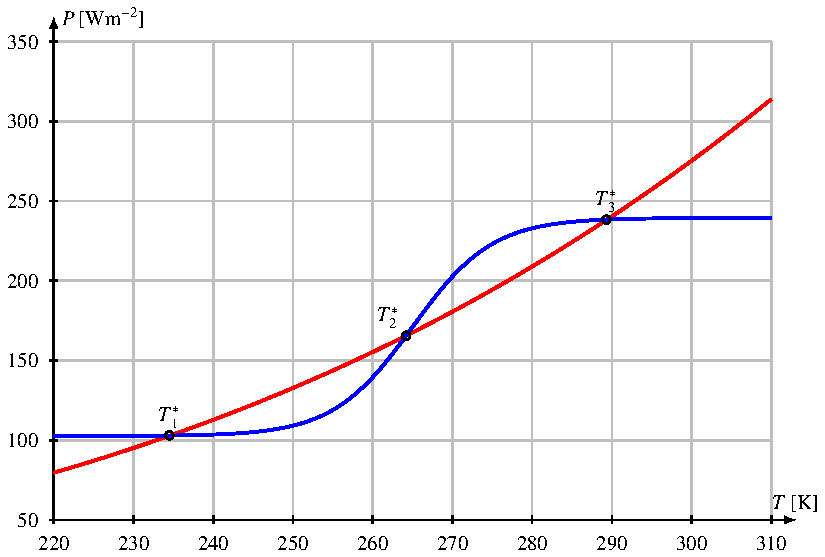
\includegraphics{chapters/5/bilanzmodell.pdf}
\caption{Einstrahlung und Ausstrahlung in dem einfachen Bilanzmodell
mit der Modellgleichung
\eqref{skript:bilanz:basic2} und der Albedo-Funktion
\eqref{skript:bilanz:albedo}.
Die Ausstrahlung $\varepsilon\sigma T^4$ ist rot eingezeichnet,
blau ist die Ausstrahlung.
Es entstehen drei Gleichgewichtspunkte $T_1^*$, $T_2^2*$ und $T_3^*$,
von denen aber $T_2^*$ nicht stabil ist.
\label{skript:bilanz:modellbild}}
\end{figure}
Das Modell mit der Albedo-Funktion~\eqref{skript:bilanz:albedo}
hat nicht nur einen sondern drei Gleichgewichtspunkte.
Die Einstrahlung und die Ausstrahlung ist in
Abbildung~\ref{skript:bilanz:modellbild} dargestellt.

Die beiden Gleichgewichtspunkte $T_1^*$ und $T_3^*$ sind stabil.
In beiden Punkten ändert sich die absorbierte Energie kaum bei
einer Temperaturänderung, aber die Ausstrahlung wird bei erhöhter 
Temperatur wesentlich effizienter, so dass sich die Erde wieder
abkühlt.
Ebenso verringert sich die Ausstrahlung bei leicht tieferer Temperatur
sofort, so dass die Erde sich wieder zur Gleichgewichtstemperatur aufwärmen
kann.

Das Gleichgewicht $T_2^*$ ist dagegen nicht stabil.
Bei höherer Temperatur wird die Einstrahlung sofort grösser, ohne dass
die Ausstrahlung mithalten kann, so dass sich die Erde weiter
aufwärmt bis zur Temperatur $T_3^*$.
Bei leicht tieferer Temperatur steigt die Albedo stark an so dass die
Einstrahlung schnell abnimmt, während die Ausstrahlung nur vergleichsweise
langsam zurückgeht, die Erde kühlt sich bis auf die Temperatur $T_1^*$ ab.

\subsubsection{Bifurkation und globale Erwärmung}
\begin{figure}
\centering
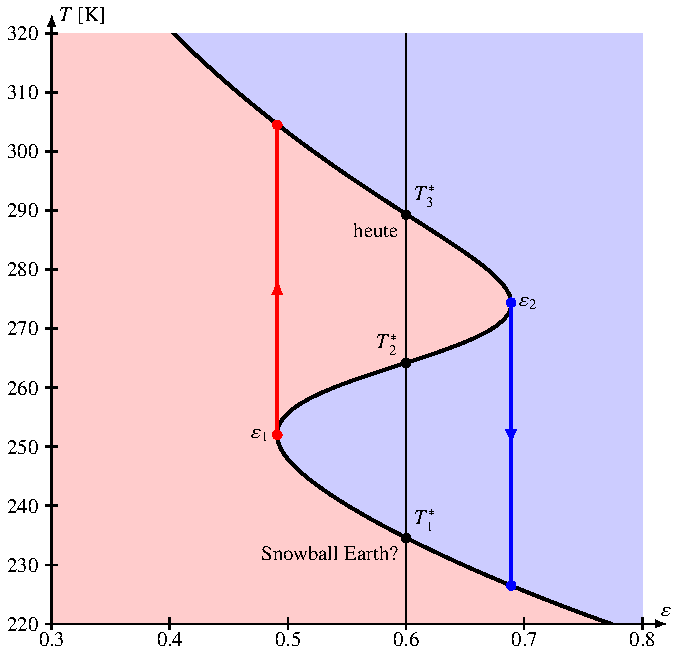
\includegraphics{chapters/5/bifurkation.pdf}
\caption{Bifurkationsdiagramm für das Bilanzmodell
\eqref{skript:bilanz:basic2}
in Abhängigkeit vom Treibhauseffekt-Parameter $\varepsilon$.
\label{skript:bilanz:bifurkation}}
\end{figure}
Der Parameter $\varepsilon$ modelliert den Treibhauseffekt.
Steigt die Konzentration der Klimagase in der Atmosphäre, wird die
abgestrahlten Leistung geringer, also $\varepsilon$ kleiner.
Es lohnt sich daher, die Entwicklung des Gleichgewichtspunkte in 
Abhängigkeit von $\varepsilon$ zu untersuchen.
Das Bifurkationsdiagramm des Modells
\eqref{skript:bilanz:basic2} in Abhängigkeit von $\varepsilon$
ist in Abbildung~\ref{skript:bilanz:bifurkation} dargestellt.

Man kann aus dem Diagramm ablesen, dass mit weitterer Zunahme des 
Treibhauseffektes, als mit Abnahme von $\varepsilon$, die globale
Mitteltemperatur weiter ansteigen wird.
Sinkt $\varepsilon$ unter den kritischen Wert $\varepsilon_1$ steigt die
Temperatur auf über $305\,\text{K}$.
In diesem Fall verschwinden die beiden Gleichgewichtspunkte $T_1^*$
und $T_2^*$, es bleibt nur das Gleichgewicht $T_3^*$.

Interessant ist aber auch, was bei starker Abnahme der
Treibhausgaskonzentration passiert.
Wenn $\varepsilon$ über $\varepsilon_2$ ansteigt, dann verschwinde
$T_3^*$ und $T_2^*$, es bleibt nur der Gleichgewichtspunkt $T_1^*$,
bei dem die ganze auf sehr tiefer Temperatur vereist.
Man vermutet, dass genau dieser Zustand in der Phase des {\em Snowball Earth}
eingetreten ist, als die ersten photosynthetisierenden Organismen die
Treibhausgase dramatische reduziert und damit $\varepsilon$ stark
erhöht hatten.
Man beachte dass es nur möglich ist, den heutigen Zustand wieder zu 
erreichen, indem die Treibhausgaskonzentration soweit gesteigert
wird, dass $\varepsilon<\varepsilon_1$ wird.
Es muss im Laufe der Erdgeschichte also nach der Snowball Earth Phase
auch Phasen mit wesentlich höherer Treibhausgaskonzentration als heute
gegeben haben.

\subsection{Modell von Budyko\label{subsection:modell von budyko}}
Bisher haben wir die Ausstrahlung mit Hilfe des Stefan-Boltzmannschen
Gesetzes für die Strahlung eines schwarzen Körpers modelliert.
Es ist fraglich, ob dies tatsächlich zutreffend ist.
Die Ausstrahlung $E_\text{out}(T)$ der Ausstrahlung könnte also durchaus
eine kompliziertere Funktion sein.
Sie muss aber so beschaffen sein, dass sich bei der aktuellen
Mitteltemperatur $T^*$ ein stabiles Gleichgewicht ergibt.
In der Umgebung des Gleichgewichtes kann die Funktion $E_\text{out}(T)$
als lineare Funktion
$E_\text{out}= A+BT$
dargestellt werden.
Nahe bei $T^*$ kann die globale Mitteltemperatur also mit einem Modell
der Form
\begin{equation}
C
\frac{dT}{dt}
=
(1-\alpha(T)) Q- (A+BT)
\end{equation}
beschrieben werden.
Das Gleichgewicht erfüllt
\[
(1-\alpha(T^*))Q=A+BT^*
\] 
und ist stabil, wenn die Steigung der Einstrahlung kleiner ist als die
Die Steigung der Ausstrahlung, also
\begin{equation}
-Q\alpha'(T)
<
B.
\label{skript:budyko:cond}
\end{equation}
Dieses Modell wurde schon in den sechziger Jahren von Budyko vorgeschlagen.
Zahlenwerte für $A$ und $B$ konnte seit der damaligen Zeit durch
Satellitenmessungen bestimmt werden.

Die Folgen des Treibhauseffektes sind auch in diesem einfacheren Modell
nachvollziehbar.
Die Erhöhung der Treibhausgaskonzentration reduziert die Ausstrahlung,
was sich zum Beispiel in einem kleineren Wert von $B$ äussert.
Eine Abnahme von $B$ um $\Delta B$ führt zu einer
Änderung der Gleichgewichtstemperatur um $\Delta T$, die die Gleichung
\begin{align*}
(1-\alpha(T^*+\Delta T))Q
&=
A + (B-\Delta B)(T^*+\Delta T)
\\
\underbrace{(1-\alpha(T^*))Q}_{\displaystyle=A+BT^*}
-Q\alpha'(T^*)\Delta T
&=
A+BT^*
- T^*\Delta B
+B\Delta T
\\
(Q\alpha'(T^*)
+
B)\Delta T
&=
T^*
\Delta B
\\
\Delta T
&=
\frac{T^*\Delta B}{Q\alpha'(T^*)+B}
\end{align*}
erfüllt.
Man kann daraus ablesen, dass eine Abnahme von $B$ genau dann zu einer
Zunahme der Mitteltemperatur, wenn der Nenner positiv ist, also
\[
Q\alpha'(T^*)+B > 0
\qquad\Rightarrow\qquad
-Q\alpha'(T^*)<B,
\]
was die Bedingung
\eqref{skript:budyko:cond}
beweist.





%
% zonen.tex -- Zonenmodelle für das Klima
%
% (c) 2018 Prof Dr Andreas Müller, Hochschule Rapperswil
%
\chapter{Zonenmodelle\label{chapter:zonenmodelle}}
\lhead{Kapitel \thechapter: Zonenmodelle}
Die Erdrotation ist schnell im Vergleich zu den für typische Klimamodelle
wesentlichen Zeitspannen.
Wesentliche Aspekte der Klimaentwicklung sollten sich daher immer
noch modellieren lassen, wenn man den Zustand des Klimasystems über
die Erdrotation mittelt.
In diesem Kapitel werden daher vereinfachte Modelle diskutiert,
die nur die geographischen Länge als geometrischen Parameter haben.

%
% strahlung.tex
%
% (c) 2018 Prof Dr Andreas Müller, Hochschule Rapperswil
%
\section{Strahlung\label{section:strahlung}}
\rhead{Strahlung}
Die von der Erde empfange Strahlung sowie die Albedo wurden bereits in
Abschnitt~\ref{skript:grundlagen:strahlung} untersucht.
Für die später in diesem Kapitel zu untersuchenden Modelle ist aber
erforderlich, die örtliche Verteilung der Strahlung auf der Erdoberfläche
genauer zu verstehen.
In diesem Abschnitt wird daher zuerst die Strahlungsleistung auf einer
Halbkugel und später auf einer Zone um einen Breitenkreis berechnet.
\input{chapters/5/halbkugel.tex}
\input{chapters/5/einstrahlung.tex}

%
% bilanz.tex -- Bilanz-Modelle
%
% (c) 2018 Prof Dr Andreas Müller, Hochschule Rapperswil
%
\section{Strahlungsbilanzmodelle\label{skript:section:budyko}}
\rhead{Strahlunbsbilanzmodelle}
Im Kapitel~\ref{chapter:wetter und klima} haben wir die physikalischen
Grundlagen der Wetter und Klimaphänomene studiert.
In diesem Abschnitt wollen wir ein einfaches Modell für die Energiebilanz
der Erde entwickeln.

\subsection{Strahlungsbilanz\label{skript:subsection:strahlungsbilanz}}
Wir formulieren ein Modell mit einer einzigen Variablen, der globalen
Mitteltemperatur $T$.
Berechnet werden soll die zeitliche Entwicklung von $T$.

\subsubsection{Einstrahlung}
Die Erde mit Radius $R$ erhält ihre Energie von der Sonne, die
den konstanten Energiefluss $S_0 = 1368 \text{W\,m}^{-2}$
einstrahlt.
Der Querschnitt der Erde ist $\pi R^2$, auf den eine Leistung von
$\pi R^2 S_0$ fällt.
Die Atmosphäre und die Weltmeere transportieren diese Energie, wir nehmen
an, sie gleichmässig über die ganze Erdoberfläche verteilt wird.
Die pro Flächeneinheit anfallende Leistung ist daher
\begin{equation}
\frac{\pi R^2 S_0}{4\pi R^2} = \frac14S_0=Q.
\label{skript:bilanz:einstrahlung}
\end{equation}

Doch kann nicht die gesamte Energie absorbiert werden.
Ein Teil wird von Wolken oder von Eis an der Oberfläche 
gleich wieder reflektiert, aber auch Landmassen und die Meere reflektieren
einen kleineren Teil der Strahlung.
Die auf Seite~\pageref{skript:subsubsection:albedo} beschriebene Albedo
hat für die Erde Werte zwischen $0.3$ und $0.7$ je nach dem Grad der
Bewölkung und der Vereisung.
Bei tieferer Temperatur muss mit stärkerer Vereisung und mehr Wolken
gerechnet werden.
Sei $\alpha(T)$ die Albedo der Erde bei der Temperatur $T$.
Der von der Erde absorbierte Fluss ist daher
\begin{equation}
(1-\alpha(T)) Q.
\label{skript:bilanz:ausstrahlung}
\end{equation}
Die Grösse $1-\alpha(T)$ heisst auch die {\em Coalbedo}.
\index{Coalbedo}%

\subsubsection{Ausstrahlung}
Die Erde verliert Energie auch wieder durch Strahlung.
Nach dem Stefan-Boltzmannschen Gesetz~\eqref{skript:stefon-boltzmann}
ist die Ausstrahlung der Erde proportional zur vierten Potenz der
Temperatur, also $T^4$.

\subsubsection{Bilanzgleichung}
Die Temperatur ändert sich umso mehr, je grösser das Ungleichgewicht
zwischen Einstrahlung \eqref{skript:bilanz:einstrahlung} und
\eqref{skript:bilanz:ausstrahlung} ist.
Die Wärmekapazität der Erdoberfläche spielt ebenfalls
eine Rolle, je grösser diese ist, desto träger folgt die Temperatur dem
Energiebilanzüberschuss.

Wir erhalten so die Differentialgleichung
\begin{equation}
C\frac{dT}{dt}
=
(1-\alpha(T)) Q - \sigma T^4.
\label{skript:bilanz:basic}
\end{equation}
Je grösser $C$ ist, desto kleiner ist die Änderungsgeschwindigkeit der
globalen Mitteltemperatur bei gleicher rechter Seite.

\subsubsection{Gleichgewichtslösung}
Wir suchen eine Gleichgewichtslösung für dieses Modell, und nehmen zu diesem
Zweck den typischen Wert $\alpha=0.3$ der Albedo der Erde.
Sie muss $\dot T=0$ erfüllen, also
\begin{align*}
(1-\alpha) Q -\sigma T^4 &=0
\\
\Rightarrow
\qquad
T&=\root 4\of{\frac{(1-\alpha)Q}{\sigma}}
\end{align*}
Setzt man die üblichen Werte für $Q$ ein, erhält man eine globale
Mitteltemperatur von $T=254.8\,\text{K}$.

\subsubsection{Treibhauseffekt}
Die tatsächliche global Mitteltemperatur $T=287.7\,\text{K}$ ist.
Diese Diskrepanz ist zwei Unzulänglichkeiten diesen einfachen
Modells zurückzuführen:
\begin{enumerate}
\item
Der Treibhauseffekt sorgt dafür, dass nur ein Teil der abgestrahlten
Wärmestrahlung die Erde tatsächlich verlässt.
Wir können dies dadurch modellieren, dass wir in der Gleichung
\eqref{skript:bilanz:basic} den Ausstrahlungsterm um einen Faktor
$\varepsilon$ reduzieren, der den Treibhauseffekt modellieren soll.
Die neue Grundgleichung wird dann
\begin{equation}
C\frac{dT}{dt}
=
(1-\alpha(T)) Q - \varepsilon\sigma T^4.
\label{skript:bilanz:basic2}
\end{equation}
Um die aktuelle Gleichgewichtstemperatur $T=287.7\,\text{K}$ von 2010
zu reproduzieren müssen wir $\varepsilon=0.32$ wählen.
\item
Die Albedo hängt von der Temperatur ab und wird mit abnehmender 
Temperatur grösser.
Bei sehr tiefen Temperaturen kann die Albedo auf bis $0.7$ steigen.
Ein einfaches Modell, welches Diesen Sachverhalt abbildet, ist
\begin{equation}
\alpha(T)=0.5-0.2\tanh\biggl(\frac{T-265}{10}\biggr)
\label{skript:bilanz:albedo}
\end{equation}
\end{enumerate}

\subsubsection{Gleichgewichte}
\begin{figure}
\centering
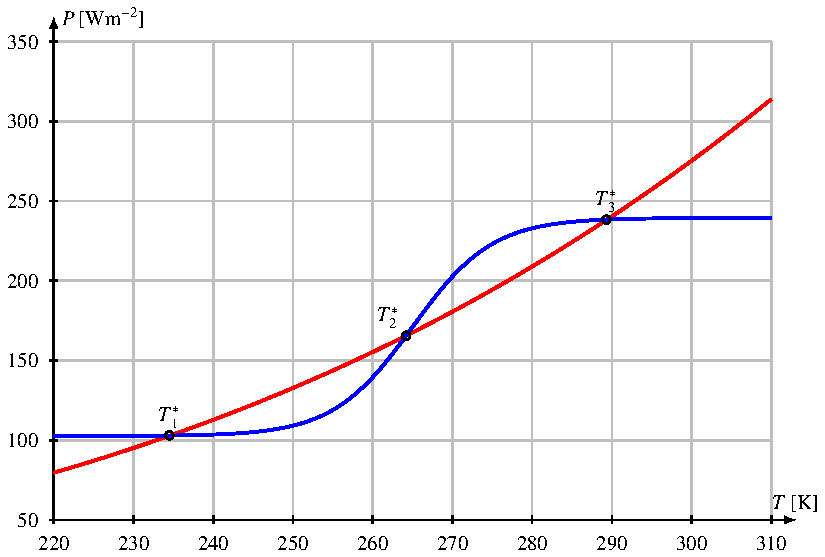
\includegraphics{chapters/5/bilanzmodell.pdf}
\caption{Einstrahlung und Ausstrahlung in dem einfachen Bilanzmodell
mit der Modellgleichung
\eqref{skript:bilanz:basic2} und der Albedo-Funktion
\eqref{skript:bilanz:albedo}.
Die Ausstrahlung $\varepsilon\sigma T^4$ ist rot eingezeichnet,
blau ist die Ausstrahlung.
Es entstehen drei Gleichgewichtspunkte $T_1^*$, $T_2^2*$ und $T_3^*$,
von denen aber $T_2^*$ nicht stabil ist.
\label{skript:bilanz:modellbild}}
\end{figure}
Das Modell mit der Albedo-Funktion~\eqref{skript:bilanz:albedo}
hat nicht nur einen sondern drei Gleichgewichtspunkte.
Die Einstrahlung und die Ausstrahlung ist in
Abbildung~\ref{skript:bilanz:modellbild} dargestellt.

Die beiden Gleichgewichtspunkte $T_1^*$ und $T_3^*$ sind stabil.
In beiden Punkten ändert sich die absorbierte Energie kaum bei
einer Temperaturänderung, aber die Ausstrahlung wird bei erhöhter 
Temperatur wesentlich effizienter, so dass sich die Erde wieder
abkühlt.
Ebenso verringert sich die Ausstrahlung bei leicht tieferer Temperatur
sofort, so dass die Erde sich wieder zur Gleichgewichtstemperatur aufwärmen
kann.

Das Gleichgewicht $T_2^*$ ist dagegen nicht stabil.
Bei höherer Temperatur wird die Einstrahlung sofort grösser, ohne dass
die Ausstrahlung mithalten kann, so dass sich die Erde weiter
aufwärmt bis zur Temperatur $T_3^*$.
Bei leicht tieferer Temperatur steigt die Albedo stark an so dass die
Einstrahlung schnell abnimmt, während die Ausstrahlung nur vergleichsweise
langsam zurückgeht, die Erde kühlt sich bis auf die Temperatur $T_1^*$ ab.

\subsubsection{Bifurkation und globale Erwärmung}
\begin{figure}
\centering
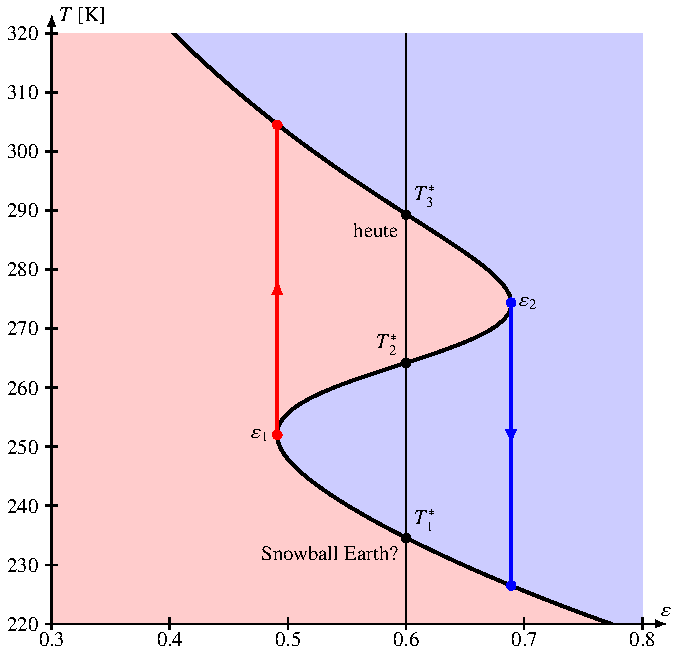
\includegraphics{chapters/5/bifurkation.pdf}
\caption{Bifurkationsdiagramm für das Bilanzmodell
\eqref{skript:bilanz:basic2}
in Abhängigkeit vom Treibhauseffekt-Parameter $\varepsilon$.
\label{skript:bilanz:bifurkation}}
\end{figure}
Der Parameter $\varepsilon$ modelliert den Treibhauseffekt.
Steigt die Konzentration der Klimagase in der Atmosphäre, wird die
abgestrahlten Leistung geringer, also $\varepsilon$ kleiner.
Es lohnt sich daher, die Entwicklung des Gleichgewichtspunkte in 
Abhängigkeit von $\varepsilon$ zu untersuchen.
Das Bifurkationsdiagramm des Modells
\eqref{skript:bilanz:basic2} in Abhängigkeit von $\varepsilon$
ist in Abbildung~\ref{skript:bilanz:bifurkation} dargestellt.

Man kann aus dem Diagramm ablesen, dass mit weitterer Zunahme des 
Treibhauseffektes, als mit Abnahme von $\varepsilon$, die globale
Mitteltemperatur weiter ansteigen wird.
Sinkt $\varepsilon$ unter den kritischen Wert $\varepsilon_1$ steigt die
Temperatur auf über $305\,\text{K}$.
In diesem Fall verschwinden die beiden Gleichgewichtspunkte $T_1^*$
und $T_2^*$, es bleibt nur das Gleichgewicht $T_3^*$.

Interessant ist aber auch, was bei starker Abnahme der
Treibhausgaskonzentration passiert.
Wenn $\varepsilon$ über $\varepsilon_2$ ansteigt, dann verschwinde
$T_3^*$ und $T_2^*$, es bleibt nur der Gleichgewichtspunkt $T_1^*$,
bei dem die ganze auf sehr tiefer Temperatur vereist.
Man vermutet, dass genau dieser Zustand in der Phase des {\em Snowball Earth}
eingetreten ist, als die ersten photosynthetisierenden Organismen die
Treibhausgase dramatische reduziert und damit $\varepsilon$ stark
erhöht hatten.
Man beachte dass es nur möglich ist, den heutigen Zustand wieder zu 
erreichen, indem die Treibhausgaskonzentration soweit gesteigert
wird, dass $\varepsilon<\varepsilon_1$ wird.
Es muss im Laufe der Erdgeschichte also nach der Snowball Earth Phase
auch Phasen mit wesentlich höherer Treibhausgaskonzentration als heute
gegeben haben.

\subsection{Modell von Budyko\label{subsection:modell von budyko}}
Bisher haben wir die Ausstrahlung mit Hilfe des Stefan-Boltzmannschen
Gesetzes für die Strahlung eines schwarzen Körpers modelliert.
Es ist fraglich, ob dies tatsächlich zutreffend ist.
Die Ausstrahlung $E_\text{out}(T)$ der Ausstrahlung könnte also durchaus
eine kompliziertere Funktion sein.
Sie muss aber so beschaffen sein, dass sich bei der aktuellen
Mitteltemperatur $T^*$ ein stabiles Gleichgewicht ergibt.
In der Umgebung des Gleichgewichtes kann die Funktion $E_\text{out}(T)$
als lineare Funktion
$E_\text{out}= A+BT$
dargestellt werden.
Nahe bei $T^*$ kann die globale Mitteltemperatur also mit einem Modell
der Form
\begin{equation}
C
\frac{dT}{dt}
=
(1-\alpha(T)) Q- (A+BT)
\end{equation}
beschrieben werden.
Das Gleichgewicht erfüllt
\[
(1-\alpha(T^*))Q=A+BT^*
\] 
und ist stabil, wenn die Steigung der Einstrahlung kleiner ist als die
Die Steigung der Ausstrahlung, also
\begin{equation}
-Q\alpha'(T)
<
B.
\label{skript:budyko:cond}
\end{equation}
Dieses Modell wurde schon in den sechziger Jahren von Budyko vorgeschlagen.
Zahlenwerte für $A$ und $B$ konnte seit der damaligen Zeit durch
Satellitenmessungen bestimmt werden.

Die Folgen des Treibhauseffektes sind auch in diesem einfacheren Modell
nachvollziehbar.
Die Erhöhung der Treibhausgaskonzentration reduziert die Ausstrahlung,
was sich zum Beispiel in einem kleineren Wert von $B$ äussert.
Eine Abnahme von $B$ um $\Delta B$ führt zu einer
Änderung der Gleichgewichtstemperatur um $\Delta T$, die die Gleichung
\begin{align*}
(1-\alpha(T^*+\Delta T))Q
&=
A + (B-\Delta B)(T^*+\Delta T)
\\
\underbrace{(1-\alpha(T^*))Q}_{\displaystyle=A+BT^*}
-Q\alpha'(T^*)\Delta T
&=
A+BT^*
- T^*\Delta B
+B\Delta T
\\
(Q\alpha'(T^*)
+
B)\Delta T
&=
T^*
\Delta B
\\
\Delta T
&=
\frac{T^*\Delta B}{Q\alpha'(T^*)+B}
\end{align*}
erfüllt.
Man kann daraus ablesen, dass eine Abnahme von $B$ genau dann zu einer
Zunahme der Mitteltemperatur, wenn der Nenner positiv ist, also
\[
Q\alpha'(T^*)+B > 0
\qquad\Rightarrow\qquad
-Q\alpha'(T^*)<B,
\]
was die Bedingung
\eqref{skript:budyko:cond}
beweist.





%
% zonen.tex -- Zonenmodelle für das Klima
%
% (c) 2018 Prof Dr Andreas Müller, Hochschule Rapperswil
%
\chapter{Zonenmodelle\label{chapter:zonenmodelle}}
\lhead{Kapitel \thechapter: Zonenmodelle}
Die Erdrotation ist schnell im Vergleich zu den für typische Klimamodelle
wesentlichen Zeitspannen.
Wesentliche Aspekte der Klimaentwicklung sollten sich daher immer
noch modellieren lassen, wenn man den Zustand des Klimasystems über
die Erdrotation mittelt.
In diesem Kapitel werden daher vereinfachte Modelle diskutiert,
die nur die geographischen Länge als geometrischen Parameter haben.

\input{chapters/5/strahlung.tex}
\input{chapters/5/bilanz.tex}
\input{chapters/5/zonen.tex}
\input{chapters/5/spektral.tex}


%
% spektral.tex -- Einführung in spektrale Methoden
%
% (c) 2018 Prof Dr Andreas Müller, Hochschule Rapperswil
%
\section{Spektrale Methoden\label{section:spektrale methoden}}
\rhead{Spektrale Methoden}
In den Ausführungen zum Lorenz-Modell in Abschnitt~\ref{section:lorenz-modell}
werden wir sehen,
wie man mit Hilfe einer geeigneten Wahl von Basisfunktionen
die komplexen fluiddynamischen partiellen Differentialgleichungen zu einem
System von gewöhnlichen Differentialgleichungen vereinfachen kann.
Die Basis wurde so gewählt, dass einerseits möglichst viel geometrische
Information, im speziellen Fall die rechteckige Form des Definitionsgebietes,
bereits darin einfliesst.
Andererseits sollen sich die wesentlichsten Eigenschaften der Lösung bereits
aus wenigen Basisfunktionen rekonstruieren lassen.
Wie Kapitel~\ref{chapter:lorenz2} zeigt, lässt sich die Idee von
Abschnitt~\ref{section:lorenz-modell} sogar maschinell in eine
immer genaueres Modell erweitern, wenn nur eine geeignete Menge
von Basisfunktionen gefunden werden kann.
Ziel diese Abschnittes ist zu illustrieren, wie so eine Basis von
Funktionen aussehen könnte, mit der man globale Modelle vereinfachen
könnte.

\input{chapters/5/kugelkoordinaten.tex}
\input{chapters/5/kugelfunktionen.tex}
\input{chapters/5/spektralegleichungen.tex}





%
% spektral.tex -- Einführung in spektrale Methoden
%
% (c) 2018 Prof Dr Andreas Müller, Hochschule Rapperswil
%
\section{Spektrale Methoden\label{section:spektrale methoden}}
\rhead{Spektrale Methoden}
In den Ausführungen zum Lorenz-Modell in Abschnitt~\ref{section:lorenz-modell}
werden wir sehen,
wie man mit Hilfe einer geeigneten Wahl von Basisfunktionen
die komplexen fluiddynamischen partiellen Differentialgleichungen zu einem
System von gewöhnlichen Differentialgleichungen vereinfachen kann.
Die Basis wurde so gewählt, dass einerseits möglichst viel geometrische
Information, im speziellen Fall die rechteckige Form des Definitionsgebietes,
bereits darin einfliesst.
Andererseits sollen sich die wesentlichsten Eigenschaften der Lösung bereits
aus wenigen Basisfunktionen rekonstruieren lassen.
Wie Kapitel~\ref{chapter:lorenz2} zeigt, lässt sich die Idee von
Abschnitt~\ref{section:lorenz-modell} sogar maschinell in eine
immer genaueres Modell erweitern, wenn nur eine geeignete Menge
von Basisfunktionen gefunden werden kann.
Ziel diese Abschnittes ist zu illustrieren, wie so eine Basis von
Funktionen aussehen könnte, mit der man globale Modelle vereinfachen
könnte.

%
% kugelkoordinaten.tex -- Kugelkoordinaten
%
% (c) 2018 Prof Dr Andreas Müller, Hochschule Rapperswil
%

\subsection{Kugelkoordinaten}
Spektrale Methoden verwenden auf entscheidende Art und Weise die
Besonderheiten des natürlichen Koordinatensystems auf der Kugeloberfläche.
In diesem Abschnitt sollen daher Kugelkoordinaten und die zugehörigen 
Differentialoperatoren genauer untersucht werden.

\subsubsection{Koordinatenumrechnung}
\index{Kugelkoordinaten}%
Wir verwenden in diesem Abschnitt Kugelkoordinaten mit der üblichen
Konvention, dass die geographische Breite als Winkel $\vartheta$
ausgehend vom Nordpol oder der $z$-Achse gemessen wird,
dass also $\vartheta\in[0,\pi]$.
Die geographische Breite wird ausgehen von der $x$-Achse als
Winkel $\varphi$ gemessen.
Schliesslich bezeichnet $r$ die Entfernung eines Punktes vom Nullpunkt.

Ein Breitenkreis zur geographischen Breite $\vartheta$ hat Radius
$r\sin\vartheta$.
Damit ergeben sich die Formeln
\begin{align*}
x
&=
r\sin\vartheta\cos\varphi
\\
y
&=
r\sin\vartheta\sin\varphi
\\
z
&=
r\cos\vartheta
\end{align*}
für die Umrechnung von Kugelkoordinaten in kartesische Koordinaten.
\index{Umrechnungsformel!Kugel-Koordinaten in kartesische Koordinaten}%

\subsubsection{Differentialoperatoren}
Das Ziel ist, den Laplace-Operator in Kugelkoordinaten auszudrücken.
Zu diesem Zweck müssen die partiellen Ableitungsoperatoren nach den
Koordinaten $x$, $y$ und $z$ durch die Operatoren
\[
\frac{\partial}{\partial r},
\;
\frac{\partial}{\partial\vartheta}
\quad\text{und}\quad
\frac{\partial}{\partial\varphi}
\]
ausgedrückt werden.

Für die Ableitungsoperatoren gilt die Kettenregel in der Form
\begin{equation}
\begin{aligned}
\frac{\partial}{\partial x}
&=
\frac{\partial r}{\partial x}\frac{\partial}{\partial r}
+
\frac{\partial\vartheta}{\partial x}\frac{\partial}{\partial\vartheta}
+
\frac{\partial\varphi}{\partial x}\frac{\partial}{\partial\varphi},
\\
\frac{\partial}{\partial y}
&=
\frac{\partial r}{\partial y}\frac{\partial}{\partial r}
+
\frac{\partial\vartheta}{\partial y}\frac{\partial}{\partial\vartheta}
+
\frac{\partial\varphi}{\partial y}\frac{\partial}{\partial\varphi},
\\
\frac{\partial}{\partial z}
&=
\frac{\partial r}{\partial z}\frac{\partial}{\partial r}
+
\frac{\partial\vartheta}{\partial z}\frac{\partial}{\partial\vartheta}
+
\frac{\partial\varphi}{\partial z}\frac{\partial}{\partial\varphi}.
\end{aligned}
\label{skript:kugel:kettenregel}
\end{equation}
Die gesuchte Darstellung der Ableitungsoperatoren läuft also darauf
hinaus, die Ableitungen von Kugelkoordinaten nach nach kartesischen
Koordinaten zu bestimmen.

Die Ableitungen von $r$ werden einfacher zur berechnen durch die
Beziehung
\[
\frac{\partial r^2}{\partial x}
=
2r\frac{\partial r}{\partial x}
\qquad\Rightarrow\qquad
\frac{\partial r}{\partial x}
=\frac1{2r}\frac{\partial r^2}{\partial x}.
\]
Da $r^2=x^2+y^2+z^2$ folgt
\begin{equation}
\begin{aligned}
\frac{\partial r}{\partial x}
&=
\frac1{2r}\frac{\partial}{\partial x}(x^2+y^2+z^2)
=
\frac1{2r}2x
=
\frac{x}{r}
=
\sin\vartheta\cos\varphi,
\\
\frac{\partial r}{\partial y}
&=
\frac1{2r}\frac{\partial}{\partial x}(x^2+y^2+z^2)
=
\frac1{2r}2y
=
\frac{y}{r}
=
\sin\vartheta\sin\varphi
\\
\text{und}
\qquad
\frac{\partial r}{\partial z}
&=
\frac1{2r}\frac{\partial}{\partial z}(x^2+y^2+z^2)
=
\frac1{2r}2z
=
\frac{z}{r}
=
\cos\vartheta.
\end{aligned}
\label{skript:kugel:rableitungen}
\end{equation}

Auf ähnliche Weise lassen sich die Ableitungen von $\vartheta$ bestimmen.
Dazu geht man aus von der Identität $z=r\cos\vartheta$ und leitet sie
nach den kartesischen Koordinaten ab:
\begin{align*}
0
=
\frac{\partial z}{\partial x}
&=
\frac{\partial r}{\partial x}\cos\vartheta
-
r\sin\vartheta\frac{\partial \vartheta}{\partial x}
&&\Rightarrow&
\frac{\partial\vartheta}{\partial x}
&=
\frac{1}{r\sin\vartheta}
\cos\vartheta
\frac{\partial r}{\partial x},
\\
0
=
\frac{\partial z}{\partial y}
&=
\frac{\partial r}{\partial y}\cos\vartheta
-
r\sin\vartheta\frac{\partial \vartheta}{\partial y}
&&\Rightarrow&
\frac{\partial \vartheta}{\partial y}
&=
\frac{1}{r\sin\vartheta}
\cos\vartheta
\frac{\partial r}{\partial y},
\\
1
=
\frac{\partial z}{\partial z}
&=
\frac{\partial r}{\partial y}\cos\vartheta
-
r\sin\vartheta\frac{\partial \vartheta}{\partial y}
&&\Rightarrow&
\frac{\partial\vartheta}{\partial y}
&=
-\frac1{r\sin\vartheta}
\biggl(1-
\cos\vartheta
\frac{\partial r}{\partial z}
\biggr).
\end{align*}
Die Ableitungen von $r$ wurden in \eqref{skript:kugel:rableitungen}
bereits berechnet, so dass wir nach den
Ableitungen von $\vartheta$ auflösen können.
Wir erhalten
\begin{equation}
\begin{aligned}
\frac{\partial\vartheta}{\partial x}
&=
\frac1{r\sin\vartheta} \cos\vartheta \sin\vartheta\cos\varphi
=
\frac{\cos\vartheta\cos\varphi}{r},
\\
\frac{\partial\vartheta}{\partial y}
&=
\frac{1}{r\sin\vartheta} \cos\vartheta \sin\vartheta\sin\varphi
=
\frac{\cos\vartheta\sin\varphi}{r},
\\
\frac{\partial\vartheta}{\partial z}
&=
-\frac{1}{r\sin\vartheta}\underbrace{(1-\cos^2\vartheta)}_{\displaystyle\sin^2\vartheta}
=
-
\frac{\sin\vartheta}r.
\end{aligned}
\label{skript:kugel:thetaableitungen}
\end{equation}
Diese Umformungen waren möglich, weil $z$ nur von $r$ und $\vartheta$ abhing.
Die Kettenregel hat dann eine Beziehung zwischen den beiden Ableitungen
dieser Variablen geliefert.

Die verbleibenden Anleitungen können auf ähnliche Weise aus dem Ausdruck
$x=r\sin\vartheta\cos\varphi$
oder
$y=r\sin\vartheta\sin\varphi$
gewonnen werden.
Wenn man ihn partiell nach kartesischen Koordinaten ableitet,
steht auf der linken Seite eine 1 oder 0,
auf der rechten Seite ein Ausdruck mit allen drei Ableitungen von
Kugelkoordinaten nach $x$, wovon die Ableitungen von $r$ und $\vartheta$
nach den kartesischen Koordinaten bereits bekannt sind.
Man kann also nach den Ableitungen von $\varphi$ auflösen.
Die etwas mühsame Berechnung liefert
\begin{equation}
\begin{aligned}
\frac{\partial \varphi}{\partial x}
&=
-\frac{\sin\varphi}{r\sin\vartheta},
\\
\frac{\partial \varphi}{\partial y}
&=
\frac{\cos\varphi}{r\sin\vartheta},
\\
\frac{\partial \varphi}{\partial z}
&=
0.
\end{aligned}
\label{skript:kugel:phiableitungen}
\end{equation}

In den Gleichungen
\eqref{skript:kugel:rableitungen},
\eqref{skript:kugel:thetaableitungen}
und
\eqref{skript:kugel:phiableitungen}
haben wir alle Koeffizienten für die Kettenregel
\eqref{skript:kugel:kettenregel}
gefunden.
Zusammen erlauben sie, Ableitungen nach kartesischen Koordinaten
durch Ableitungen nach Kugelkoordinaten auszudrücken.

\subsubsection{Laplace-Operator}
In kartesischen Koordinaten ist der Laplace-Operator gegeben durch die
Definition
\[
\Delta
=
\frac{\partial^2}{\partial x^2}
+
\frac{\partial^2}{\partial y^2}
+
\frac{\partial^2}{\partial z^2}.
\]
Durch Einsetzen der Ableitungsoperatoren nach
\eqref{skript:kugel:kettenregel} unter Verwendung der Gleichungen
\eqref{skript:kugel:rableitungen},
\eqref{skript:kugel:thetaableitungen}
und
\eqref{skript:kugel:phiableitungen}
kann man nach ziemlich langwieriger
Rechnung~\cite[Anhang B.3]{skript:mathsem-qm}
den Ausdruck
\begin{equation}
\Delta
=
\frac1{r^2}\frac{\partial}{\partial r}
\biggl(r^2\frac{\partial}{\partial r}\biggr)
+
\frac{1}{r^2\sin\vartheta}\frac{\partial}{\partial\vartheta}
\biggl(\sin\vartheta\frac{\partial}{\partial\vartheta}\biggr)
+
\frac{1}{r^2}
\frac{1}{\sin^2\vartheta}
\frac{\partial^2}{\partial\varphi^2}.
\end{equation}
für den Laplace-Operator in Kugelkoordinaten finden.
\index{Laplace-Operator in Kugelkoordinaten}%


%
% kugelfunktionen.tex -- Kugelfunktionen
%
% (c) 2018 Prof Dr Andreas Müller, Hochschule Rapperswil
%
\subsection{Kugelfunktionen}
Die Basisfunktionen im Lorenz-Modell waren aus zwei Gründen besonders
erfolgreich.
\begin{enumerate}
\item
Die Basisfunktionen waren Produkte von Funktionen, die jeweils nur von
einer Koordinate abhängen.
In einem Produkt 
$f(x,y)=X(x)\cdot Y(y)$ 
sind die Ableitungen nach den Koordinaten besonders einfach auszurechnen,
da gilt
\[
\begin{aligned}
\frac{\partial f}{\partial x}(x,y) &= X'(x)\cdot Y(y)
&&\text{und}&
\frac{\partial f}{\partial y}(x,y) &= X(x)\cdot Y'(y).
\end{aligned}
\]
\item
Die Basisfunktionen waren Eigenfunktionen des Laplace-Operators, also
\[
\Delta f = \lambda f.
\]
Da in den Gleichungen der Strömungsdynamik der Laplace-Operator
prominent vorkommt, bedeutet diese Eigenschaft, dass die Wirkung des
Laplace-Operators auf die Basisfunktionen durch Multiplikation mit
dem Eigenwert ersetzt werden kann.
Dadurch werden die Gleichungen sehr vereinfacht und die Ordnung
der Differentialgleichung reduziert sich.
\end{enumerate}
Wenn der Erfolg der speziellen Basiswahl im Lorenz-System für ein
Wetter- oder Klimamodell auf der Kugeloberfläche repliziert werden
soll, dann ist nahe liegend, dass dazu Funktionen mit den gleichen
Eigenschaften in Kugelkoordinaten gefunden werden müssen.

\subsubsection{Separationsansatz}
Die Produkteigenschaft bedeutet, dass die Basisfunktionen in der Form
\[
f(r,\varphi,\vartheta)
=
R(r)\cdot \Phi(\varphi)\cdot \Theta(\vartheta)
\]
gefunden werden müssen.
Das in Abschnitt~\ref{section:pdeloesungen} dargestellte
Separationsverfahren für partielle
Differentialgleichungen~\cite[Chapter 4]{skript:pde}
basiert genau auf dieser Art von Ansatz.

\subsubsection{Eigenwertgleichung}
Die Eigenwerteigenschaft bedeutet, dass die Funktionen Eigenfunktionen
des Laplace-Operators sein müssen, also Lösungen der partiellen
Differentialgleichungen
\[
\Delta f = \lambda f.
\]
Wenden wir den Laplace-Operator in Kugelkoordinaten auf $f$ an, finden
wir
\begin{align*}
\Delta f
&=
\biggl(
\frac{1}{r^2} \frac{\partial}{\partial r}
\biggl(r^2\frac{\partial f}{\partial r}\biggr)
+
\frac1{r^2\sin\vartheta}\frac{\partial}{\partial\vartheta}
\biggl(\sin\vartheta\frac{\partial f}{\partial\vartheta}\biggr)
+
\frac1{r^2\sin^2\vartheta}\frac{\partial^2 f}{\partial\varphi^2}
\biggr)
R(r)\cdot \Phi(\varphi)\cdot \Theta(\vartheta)
\\
&=
\frac1{r^2}\frac{\partial}{\partial r}\bigl(r^2R'(r)\bigr)
\cdot \Theta(\vartheta)\cdot \Phi(\varphi)
+
\frac1{r^2\sin\vartheta}\frac{d}{d\vartheta}
\bigl(\sin\vartheta \Theta'(\vartheta)\bigr)
\cdot R(r)\cdot \Phi(\varphi)
\\
&\qquad
+
\frac1{r^2\sin^2\vartheta}\Phi''(\varphi)
\cdot R(r)\cdot \Theta(\vartheta)
\\
&=
\frac1{r^2}\bigl(2rR'(r)+r^2R''(r)\bigr)
\Theta(\vartheta)\Phi(\varphi)
+
\frac1{r^2\sin\vartheta}
\bigl(\sin\vartheta\Theta'(\vartheta)\bigr)'
\cdot R(r)\cdot\Phi(\varphi)
\\
&\qquad
+
\frac1{r^2\sin^2\vartheta}
\Phi''(\varphi)
\cdot R(r)\cdot \Theta(\vartheta)
\\
&=
\lambda
R(r)\cdot \Theta(\vartheta)\cdot \Phi(\varphi).
\end{align*}

\subsubsection{Separation von $r$}
Um die einzelnen Funktionen zu isolieren, teilen wir durch $f$.
Zwar kann $f$ Nullstellen haben, aber für die meisten Werte der Koordinaten
ist $f$ von Null verschieden, für diese Punkte ist die Division unproblematisch
und ausreichend, um die Faktoren zu bestimmen.
Wir erhalten
\begin{align*}
\frac{2rR'(r)+r^2R''(r)}{r^2R(r)}
+
\frac{
\bigl(\sin\vartheta\Theta'(\vartheta)\bigr)'
}{r^2\sin\vartheta\Theta(\vartheta)}
+
\frac{1}{r^2\sin^2\vartheta}\frac{\Phi''(\varphi)}{\Phi(\varphi)}
&=\lambda
\end{align*}
Um die Variable $r$ allein auf die linke Seite zu bringen, multiplizieren wir
mit $r^2$, subtrahieren $\lambda r^2$ und bringen den zweiten und dritten 
Term auf der linken Seite auf die rechte Seite.
So erhalten wir
\begin{align*}
\frac{r^2R''(r)+2rR'(r)-\lambda r^2R(r)}{R(r)}
&=
-
\frac{
\bigl(\sin\vartheta\,\Theta'(\vartheta)\bigr)'
}{\sin\vartheta\,\Theta(\vartheta)}
-\frac{1}{\sin^2\vartheta}\frac{\Phi''(\varphi)}{\Phi(\varphi)}
\end{align*}
Die linke Seite hängt nur von $r$ ab, die rechte Seite nur von $\vartheta$
und $\varphi$.
Dies ist nur möglich, wenn beide Seiten konstant sind.
Es gibt also ein Zahl $\mu$ derart, dass
\begin{align}
\frac{r^2R''(r)+2rR'(r)-\lambda r^2R(r)}{R(r)}&=\mu,
\\
\frac{\bigl(\sin\vartheta\,\Theta'(\vartheta)\bigr)'}{\sin\vartheta\,\Theta(\vartheta)}
+
\frac{1}{\sin^2\vartheta}\frac{\Phi''(\varphi)}{\Phi(\varphi)}
&=
-\mu.
\label{skript:kugel:thetaphi}
\end{align}
Die erste Gleichung kann man vereinfachen zu
\begin{equation}
r^2R''(r)+2rR'(r)-(\lambda r^2-\mu)R(r) = 0,
\end{equation}
eine gewöhnliche lineare Differentialgleichung zweiter Ordnung.
$\mu$ kann nicht beliebig gewählt werden, der Wert muss so sein,
dass \eqref{skript:kugel:thetaphi} gelöst werden kann.

Doch auch $\lambda$ ist nicht beliebig, sein Wert muss so gewählt
werden, dass eventuelle Randbedingungen für die zugehörigen Funktion
$R(r)$ erfüllt sind.
Da die $r$-Abhängigkeit für die folgende Diskussion nicht wichtig ist,
verfolgen wir diese Frage hier nicht weiter.

\subsubsection{Separation von $\vartheta$ und $\varphi$}
Die Gleichung~\eqref{skript:kugel:thetaphi} enthält nur noch die
Variablen $\vartheta$ und $\varphi$. 
Wir versuchen den gleichen Trick erneut: indem wir mit $\sin^2\vartheta$
multiplizieren, den Term mit $\mu$ auf die linke Seite bringen und
den zweiten Term auf die rechte Seite bringen, erhalten wir
\[
\sin\vartheta
\frac{1}{\Theta(\vartheta)}
\frac{d}{d\vartheta}\bigl(\sin\vartheta\,\Theta'(\vartheta)\bigr)
+
\mu\sin^2\vartheta
=
-\frac{\Phi''(\varphi)}{\Phi(\varphi)}.
\]
Erneut haben wir eine Gleichung, deren linke Seite nur von $\vartheta$
und deren rechte Seite nur von $\varphi$ abhängt.
Also sind wieder beide Seiten konstant, es gibt also eine Konstante
$\nu$ derart, dass $\Theta(\vartheta)$ und $\Phi(\varphi)$ die 
Gleichungen
\begin{align}
\sin\vartheta\frac{d}{d\vartheta}
\biggl(
\sin\vartheta\frac{d}{d\vartheta}\Theta(\vartheta)
\biggr)
&=
(-\mu\sin^2\vartheta+\nu)\Theta(\vartheta)
\label{skript:kugel:thetagl}
\\
-\frac{\Phi''(\varphi)}{\Phi(\varphi)}&=\nu
\label{skript:kugel:phigl}
\end{align}
erfüllen.

\subsubsection{Lösungsfunktionen $\Phi(\varphi)$}
Die zweite Gleichung~\eqref{skript:kugel:phigl} ist gleichbedeutend mit
\begin{equation}
\Phi''(\varphi)=-\nu\Phi(\varphi),
\label{skript:kugel:philsg}
\end{equation}
wobei $\Phi(\varphi)$ eine $2\pi$-periodische Funktion ist.
Die Lösungen der Gleichung~\eqref{skript:kugel:philsg}
sind $\cos\sqrt{\nu}\varphi$ und $\sin\sqrt{\nu}\varphi$,
aber die Periodizität verlangt, dass $\sqrt{\nu}$ eine ganze Zahl ist.
Es muss also gelten $\nu=k^2$ mit $k\in \mathbb N$.

\subsubsection{Lösungsfunktionen $\Theta(\vartheta)$}
Im vorangegangen Absatz wurde gezeigt, dass $\nu=k^2$ ist, was die
Gleichung~\eqref{skript:kugel:thetagl} zu
\begin{equation}
\sin\vartheta\frac{d}{d\vartheta}\sin\vartheta\frac{d}{d\vartheta}\Theta(\vartheta)
=
\biggl(\sin\vartheta\frac{d}{d\vartheta}\biggr)^2 \Theta(\vartheta)
=
(-\mu\sin^2\vartheta+k^2)\Theta(\vartheta)
\label{skript:kugel:legendredgl0}
\end{equation}
In dieser Form ist die Differentialgleichung nicht so leicht zu
erkennen.
Schreibt man aber $z=\sin\vartheta$, dann wird die Ableitung einer
Funktion $P(z)=\Theta(\vartheta)$
\begin{align*}
\frac{d}{d\vartheta}\Theta(\vartheta)
=
\frac{d}{d\vartheta}P(\cos\vartheta)
=
-P'(\cos\vartheta) \sin\vartheta
&=
-\sqrt{1-\cos^2\vartheta}P'(\cos\vartheta)
\\
&=
-\sqrt{1-z^2}P'(z)
=
-\sqrt{1-z^2}\frac{d}{dz}P(z).
\end{align*}
Ableitungen nach $\vartheta$ sind also zu ersetzen durch Ableitungen
nach $z$ gefolgt von Multiplikation mit $-\sqrt{1-z^2}$.
In der Differentialgleichung~\eqref{skript:kugel:legendredgl0}
wird die Ableitung nach $\vartheta$ jeweils auch noch mit $\sin\vartheta=\sqrt{1-z^2}$
multipliziert.
Der Operator
\begin{equation}
\sin\vartheta\frac{d}{d\vartheta}
\qquad
\text{bekommt daher die Form}
\qquad
-(1-z^2)\frac{d}{dz}.
\label{skript:kugel:zoperator}
\end{equation}
Das Vorzeichen ist nicht wichtig, da der Operator in der Differentialgleichung
\eqref{skript:kugel:legendredgl0} nur im Quadrat vorkommt.

Wir setzen jetzt die Form \eqref{skript:kugel:zoperator}
des Differentialoperators in die Differentialgleichung
\eqref{skript:kugel:legendredgl0} ein
und erhalten 
\begin{align}
(1-z^2)\frac{d}{dz}\bigl((1-z^2)P'(z)\bigr)
&=
(-\mu(1-z^2)+m^2)P(z)
\notag
\\
\Rightarrow\qquad
(1-z^2)P''(z) -2z P'(z)
+
\mu P(z)
-\frac{m^2}{1-z^2}P(z)
&=
0.
\label{skript:kugel:legendredgl}
\end{align}
Für $m=0$ ist
\eqref{skript:kugel:legendredgl}
die sogenannte Legendresche Differentialgleichung.
\index{Differentialgleichung!Legendresche}
\index{Legendresche Differentialgleichung}
Sie hat Lösungen für $\mu=l(l+1)$ mit $l\in\mathbb N$.
Für $m>0$ ist
\eqref{skript:kugel:legendredgl}
die assozierte Legendre-Differentialgleichung.
Für beide Gleichung lassen sich Lösungen angeben, es sind die
sogenannten Legendre-Polynome $P_l(z)$ im Fall $m=0$ und die zugeordneten
Legendre-Polynome $P_l^m(z)$ für beliebiges $m$.

\subsubsection{Kugelflächenfunktionen}
Mit den gefundenen Lösungen für $\Phi(\varphi)$ und $\Theta(\vartheta)$
finden wir jetzt die allgemeinen Lösungen 
der Differentialgleichung \eqref{skript:kugel:thetaphi}.
Es sind die Funktionen
\[
Y_l^m(\vartheta,\varphi)
=
N_{lm}
P_l^m(\cos\vartheta) e^{im\varphi}
\]
mit einem geeigneten Normierungsfaktor $N_{lm}$.
Diese Funktionen haben genau die Eigenschaften, die wir in der Einleitung
dieses Abschnitts als Voraussetzungen für eine geeignete Basis
gefordert haben.




%
% spektralegleichungen.tex
%
% (c) 2018 Prof Dr Andreas Müller, Hochschule Rapperswil
%
\subsection{Spektrale Gleichungen\label{subsection:spektrale gleichungen}}
Mit den Kugelfunktionen steht jetzt eine Basis für Funktionen auf der
Kugeloberfläche oder auch für eine Kugelschicht wie die Atmosphäre zur
Verfügung.
Um die zeitliche Entwicklung zu verstehen, wie sie zum Beispiel vom
Modell~\eqref{skript:psidgl} beschrieben wird, müssen diese Gleichungen
umformuliert werden als Gleichungen für die Koeffizienten einer Darstellung
der Lösungsfunktion als Linearkombination 

Um das Prinzip zu veranschaulichen, wird dies für die Wärmeleitungsgleichung
\[
\frac{\partial T}{\partial t}
=
\kappa \Delta T
\]
auf der Kugeloberfläche gezeigt.
Die Temperatur kann also als Linearkombination
\begin{equation}
T(t, \vartheta, \varphi)
=
\sum_{l=0}^\infty \sum_{m=-l}^{l} a_{lm}(t) Y^m_l(\vartheta,\varphi)
\label{skript:spektral:ansatz}
\end{equation}
geschrieben werden.
Die Funtionen $Y^m_l(\vartheta,\varphi)$ sind nach Konstruktion
Eigenfunktionen des Laplace-Operators, der zugehörige Eigenwert soll
mit $\lambda^m_l$ abgekürzt werden.

Setzt man \eqref{skript:spektral:ansatz} in die Differentialgleichung
ein, wird sie zu
\begin{align*}
\frac{\partial T}{\partial t}
&=
\sum_{l=0}^\infty \sum_{m=-l}^{l} \frac{\partial a_{lm}(t)}{\partial t} Y^m_l(\vartheta,\varphi)
=
\sum_{l=0}^\infty \sum_{m=-l}^{l} \dot a_{lm}(t) Y^m_l(\vartheta,\varphi)
\\
\kappa\Delta T
&=
\kappa
\sum_{l=0}^\infty \sum_{m=-l}^{l} a_{lm}(t) \Delta Y^m_l(\vartheta,\varphi)
=
\kappa
\sum_{l=0}^\infty \sum_{m=-l}^{l} a_{lm}(t) \lambda^m_l Y^m_l(\vartheta,\varphi)
\end{align*}
Mittels Koeffizientenvergleich folgen die gewöhnlichen
Differentialgleichungen
\[
\dot a_{lm}(t)
=
\kappa\lambda^m_l
a_{lm},
\]
deren Lösungen man sofort angeben kann, sie sind
\[
a_{lm}(t)
=
a_{lm}(0) e^{\kappa\lambda^m_l t}.
\]
Damit kann man die Lösung der Wärmeleitungsgleichung sofort hinschreiben,
sie ist
\begin{equation}
T(t,\vartheta,\varphi)
=
\sum_{l=0}^\infty \sum_{m=-l}^{l}
a_{lm}(0) e^{\kappa\lambda^m_l t}
Y^m_l(\vartheta,\varphi).
\end{equation}
Die Verwendung der Basis der Kugelfunktionen hat also zu einer besonders 
einfachen Lösung geführt.

Die Gleichung~\eqref{skript:psidgl} ist nicht linear, die Lösung
der Gleichung wird nicht mehr so einfach sein wie im Fall der
Wärmeleitungsgleichung.
Da aber die Kugelfunktionen eine Basis bilden, müssen sich auch
Produkte von Kugelfunktionen oder Ableitungen von Kugelfunktionen
als Linearkombinationen von Kugelfunktionen ausdrücken lassen,
wie das im Beispiel auf Seite~\pageref{subsubsection:komplexeres}
für die nichtlineare Gleichung von Burgers und die Basis der
Exponentialfunktionen vorgeführt wurde.
Auch auf der Kugeloberfläche lässt sich daher ein System von gewöhnlichen
Differentialgleichungen für die Koeffizienten $a_{lm}(t)$ aufstellen,
mit dem Unterschied, dass sie nicht mehr linear sein werden.













%
% spektral.tex -- Einführung in spektrale Methoden
%
% (c) 2018 Prof Dr Andreas Müller, Hochschule Rapperswil
%
\section{Spektrale Methoden\label{section:spektrale methoden}}
\rhead{Spektrale Methoden}
In den Ausführungen zum Lorenz-Modell in Abschnitt~\ref{section:lorenz-modell}
werden wir sehen,
wie man mit Hilfe einer geeigneten Wahl von Basisfunktionen
die komplexen fluiddynamischen partiellen Differentialgleichungen zu einem
System von gewöhnlichen Differentialgleichungen vereinfachen kann.
Die Basis wurde so gewählt, dass einerseits möglichst viel geometrische
Information, im speziellen Fall die rechteckige Form des Definitionsgebietes,
bereits darin einfliesst.
Andererseits sollen sich die wesentlichsten Eigenschaften der Lösung bereits
aus wenigen Basisfunktionen rekonstruieren lassen.
Wie Kapitel~\ref{chapter:lorenz2} zeigt, lässt sich die Idee von
Abschnitt~\ref{section:lorenz-modell} sogar maschinell in eine
immer genaueres Modell erweitern, wenn nur eine geeignete Menge
von Basisfunktionen gefunden werden kann.
Ziel diese Abschnittes ist zu illustrieren, wie so eine Basis von
Funktionen aussehen könnte, mit der man globale Modelle vereinfachen
könnte.

%
% kugelkoordinaten.tex -- Kugelkoordinaten
%
% (c) 2018 Prof Dr Andreas Müller, Hochschule Rapperswil
%

\subsection{Kugelkoordinaten}
Spektrale Methoden verwenden auf entscheidende Art und Weise die
Besonderheiten des natürlichen Koordinatensystems auf der Kugeloberfläche.
In diesem Abschnitt sollen daher Kugelkoordinaten und die zugehörigen 
Differentialoperatoren genauer untersucht werden.

\subsubsection{Koordinatenumrechnung}
\index{Kugelkoordinaten}%
Wir verwenden in diesem Abschnitt Kugelkoordinaten mit der üblichen
Konvention, dass die geographische Breite als Winkel $\vartheta$
ausgehend vom Nordpol oder der $z$-Achse gemessen wird,
dass also $\vartheta\in[0,\pi]$.
Die geographische Breite wird ausgehen von der $x$-Achse als
Winkel $\varphi$ gemessen.
Schliesslich bezeichnet $r$ die Entfernung eines Punktes vom Nullpunkt.

Ein Breitenkreis zur geographischen Breite $\vartheta$ hat Radius
$r\sin\vartheta$.
Damit ergeben sich die Formeln
\begin{align*}
x
&=
r\sin\vartheta\cos\varphi
\\
y
&=
r\sin\vartheta\sin\varphi
\\
z
&=
r\cos\vartheta
\end{align*}
für die Umrechnung von Kugelkoordinaten in kartesische Koordinaten.
\index{Umrechnungsformel!Kugel-Koordinaten in kartesische Koordinaten}%

\subsubsection{Differentialoperatoren}
Das Ziel ist, den Laplace-Operator in Kugelkoordinaten auszudrücken.
Zu diesem Zweck müssen die partiellen Ableitungsoperatoren nach den
Koordinaten $x$, $y$ und $z$ durch die Operatoren
\[
\frac{\partial}{\partial r},
\;
\frac{\partial}{\partial\vartheta}
\quad\text{und}\quad
\frac{\partial}{\partial\varphi}
\]
ausgedrückt werden.

Für die Ableitungsoperatoren gilt die Kettenregel in der Form
\begin{equation}
\begin{aligned}
\frac{\partial}{\partial x}
&=
\frac{\partial r}{\partial x}\frac{\partial}{\partial r}
+
\frac{\partial\vartheta}{\partial x}\frac{\partial}{\partial\vartheta}
+
\frac{\partial\varphi}{\partial x}\frac{\partial}{\partial\varphi},
\\
\frac{\partial}{\partial y}
&=
\frac{\partial r}{\partial y}\frac{\partial}{\partial r}
+
\frac{\partial\vartheta}{\partial y}\frac{\partial}{\partial\vartheta}
+
\frac{\partial\varphi}{\partial y}\frac{\partial}{\partial\varphi},
\\
\frac{\partial}{\partial z}
&=
\frac{\partial r}{\partial z}\frac{\partial}{\partial r}
+
\frac{\partial\vartheta}{\partial z}\frac{\partial}{\partial\vartheta}
+
\frac{\partial\varphi}{\partial z}\frac{\partial}{\partial\varphi}.
\end{aligned}
\label{skript:kugel:kettenregel}
\end{equation}
Die gesuchte Darstellung der Ableitungsoperatoren läuft also darauf
hinaus, die Ableitungen von Kugelkoordinaten nach nach kartesischen
Koordinaten zu bestimmen.

Die Ableitungen von $r$ werden einfacher zur berechnen durch die
Beziehung
\[
\frac{\partial r^2}{\partial x}
=
2r\frac{\partial r}{\partial x}
\qquad\Rightarrow\qquad
\frac{\partial r}{\partial x}
=\frac1{2r}\frac{\partial r^2}{\partial x}.
\]
Da $r^2=x^2+y^2+z^2$ folgt
\begin{equation}
\begin{aligned}
\frac{\partial r}{\partial x}
&=
\frac1{2r}\frac{\partial}{\partial x}(x^2+y^2+z^2)
=
\frac1{2r}2x
=
\frac{x}{r}
=
\sin\vartheta\cos\varphi,
\\
\frac{\partial r}{\partial y}
&=
\frac1{2r}\frac{\partial}{\partial x}(x^2+y^2+z^2)
=
\frac1{2r}2y
=
\frac{y}{r}
=
\sin\vartheta\sin\varphi
\\
\text{und}
\qquad
\frac{\partial r}{\partial z}
&=
\frac1{2r}\frac{\partial}{\partial z}(x^2+y^2+z^2)
=
\frac1{2r}2z
=
\frac{z}{r}
=
\cos\vartheta.
\end{aligned}
\label{skript:kugel:rableitungen}
\end{equation}

Auf ähnliche Weise lassen sich die Ableitungen von $\vartheta$ bestimmen.
Dazu geht man aus von der Identität $z=r\cos\vartheta$ und leitet sie
nach den kartesischen Koordinaten ab:
\begin{align*}
0
=
\frac{\partial z}{\partial x}
&=
\frac{\partial r}{\partial x}\cos\vartheta
-
r\sin\vartheta\frac{\partial \vartheta}{\partial x}
&&\Rightarrow&
\frac{\partial\vartheta}{\partial x}
&=
\frac{1}{r\sin\vartheta}
\cos\vartheta
\frac{\partial r}{\partial x},
\\
0
=
\frac{\partial z}{\partial y}
&=
\frac{\partial r}{\partial y}\cos\vartheta
-
r\sin\vartheta\frac{\partial \vartheta}{\partial y}
&&\Rightarrow&
\frac{\partial \vartheta}{\partial y}
&=
\frac{1}{r\sin\vartheta}
\cos\vartheta
\frac{\partial r}{\partial y},
\\
1
=
\frac{\partial z}{\partial z}
&=
\frac{\partial r}{\partial y}\cos\vartheta
-
r\sin\vartheta\frac{\partial \vartheta}{\partial y}
&&\Rightarrow&
\frac{\partial\vartheta}{\partial y}
&=
-\frac1{r\sin\vartheta}
\biggl(1-
\cos\vartheta
\frac{\partial r}{\partial z}
\biggr).
\end{align*}
Die Ableitungen von $r$ wurden in \eqref{skript:kugel:rableitungen}
bereits berechnet, so dass wir nach den
Ableitungen von $\vartheta$ auflösen können.
Wir erhalten
\begin{equation}
\begin{aligned}
\frac{\partial\vartheta}{\partial x}
&=
\frac1{r\sin\vartheta} \cos\vartheta \sin\vartheta\cos\varphi
=
\frac{\cos\vartheta\cos\varphi}{r},
\\
\frac{\partial\vartheta}{\partial y}
&=
\frac{1}{r\sin\vartheta} \cos\vartheta \sin\vartheta\sin\varphi
=
\frac{\cos\vartheta\sin\varphi}{r},
\\
\frac{\partial\vartheta}{\partial z}
&=
-\frac{1}{r\sin\vartheta}\underbrace{(1-\cos^2\vartheta)}_{\displaystyle\sin^2\vartheta}
=
-
\frac{\sin\vartheta}r.
\end{aligned}
\label{skript:kugel:thetaableitungen}
\end{equation}
Diese Umformungen waren möglich, weil $z$ nur von $r$ und $\vartheta$ abhing.
Die Kettenregel hat dann eine Beziehung zwischen den beiden Ableitungen
dieser Variablen geliefert.

Die verbleibenden Anleitungen können auf ähnliche Weise aus dem Ausdruck
$x=r\sin\vartheta\cos\varphi$
oder
$y=r\sin\vartheta\sin\varphi$
gewonnen werden.
Wenn man ihn partiell nach kartesischen Koordinaten ableitet,
steht auf der linken Seite eine 1 oder 0,
auf der rechten Seite ein Ausdruck mit allen drei Ableitungen von
Kugelkoordinaten nach $x$, wovon die Ableitungen von $r$ und $\vartheta$
nach den kartesischen Koordinaten bereits bekannt sind.
Man kann also nach den Ableitungen von $\varphi$ auflösen.
Die etwas mühsame Berechnung liefert
\begin{equation}
\begin{aligned}
\frac{\partial \varphi}{\partial x}
&=
-\frac{\sin\varphi}{r\sin\vartheta},
\\
\frac{\partial \varphi}{\partial y}
&=
\frac{\cos\varphi}{r\sin\vartheta},
\\
\frac{\partial \varphi}{\partial z}
&=
0.
\end{aligned}
\label{skript:kugel:phiableitungen}
\end{equation}

In den Gleichungen
\eqref{skript:kugel:rableitungen},
\eqref{skript:kugel:thetaableitungen}
und
\eqref{skript:kugel:phiableitungen}
haben wir alle Koeffizienten für die Kettenregel
\eqref{skript:kugel:kettenregel}
gefunden.
Zusammen erlauben sie, Ableitungen nach kartesischen Koordinaten
durch Ableitungen nach Kugelkoordinaten auszudrücken.

\subsubsection{Laplace-Operator}
In kartesischen Koordinaten ist der Laplace-Operator gegeben durch die
Definition
\[
\Delta
=
\frac{\partial^2}{\partial x^2}
+
\frac{\partial^2}{\partial y^2}
+
\frac{\partial^2}{\partial z^2}.
\]
Durch Einsetzen der Ableitungsoperatoren nach
\eqref{skript:kugel:kettenregel} unter Verwendung der Gleichungen
\eqref{skript:kugel:rableitungen},
\eqref{skript:kugel:thetaableitungen}
und
\eqref{skript:kugel:phiableitungen}
kann man nach ziemlich langwieriger
Rechnung~\cite[Anhang B.3]{skript:mathsem-qm}
den Ausdruck
\begin{equation}
\Delta
=
\frac1{r^2}\frac{\partial}{\partial r}
\biggl(r^2\frac{\partial}{\partial r}\biggr)
+
\frac{1}{r^2\sin\vartheta}\frac{\partial}{\partial\vartheta}
\biggl(\sin\vartheta\frac{\partial}{\partial\vartheta}\biggr)
+
\frac{1}{r^2}
\frac{1}{\sin^2\vartheta}
\frac{\partial^2}{\partial\varphi^2}.
\end{equation}
für den Laplace-Operator in Kugelkoordinaten finden.
\index{Laplace-Operator in Kugelkoordinaten}%


%
% kugelfunktionen.tex -- Kugelfunktionen
%
% (c) 2018 Prof Dr Andreas Müller, Hochschule Rapperswil
%
\subsection{Kugelfunktionen}
Die Basisfunktionen im Lorenz-Modell waren aus zwei Gründen besonders
erfolgreich.
\begin{enumerate}
\item
Die Basisfunktionen waren Produkte von Funktionen, die jeweils nur von
einer Koordinate abhängen.
In einem Produkt 
$f(x,y)=X(x)\cdot Y(y)$ 
sind die Ableitungen nach den Koordinaten besonders einfach auszurechnen,
da gilt
\[
\begin{aligned}
\frac{\partial f}{\partial x}(x,y) &= X'(x)\cdot Y(y)
&&\text{und}&
\frac{\partial f}{\partial y}(x,y) &= X(x)\cdot Y'(y).
\end{aligned}
\]
\item
Die Basisfunktionen waren Eigenfunktionen des Laplace-Operators, also
\[
\Delta f = \lambda f.
\]
Da in den Gleichungen der Strömungsdynamik der Laplace-Operator
prominent vorkommt, bedeutet diese Eigenschaft, dass die Wirkung des
Laplace-Operators auf die Basisfunktionen durch Multiplikation mit
dem Eigenwert ersetzt werden kann.
Dadurch werden die Gleichungen sehr vereinfacht und die Ordnung
der Differentialgleichung reduziert sich.
\end{enumerate}
Wenn der Erfolg der speziellen Basiswahl im Lorenz-System für ein
Wetter- oder Klimamodell auf der Kugeloberfläche repliziert werden
soll, dann ist nahe liegend, dass dazu Funktionen mit den gleichen
Eigenschaften in Kugelkoordinaten gefunden werden müssen.

\subsubsection{Separationsansatz}
Die Produkteigenschaft bedeutet, dass die Basisfunktionen in der Form
\[
f(r,\varphi,\vartheta)
=
R(r)\cdot \Phi(\varphi)\cdot \Theta(\vartheta)
\]
gefunden werden müssen.
Das in Abschnitt~\ref{section:pdeloesungen} dargestellte
Separationsverfahren für partielle
Differentialgleichungen~\cite[Chapter 4]{skript:pde}
basiert genau auf dieser Art von Ansatz.

\subsubsection{Eigenwertgleichung}
Die Eigenwerteigenschaft bedeutet, dass die Funktionen Eigenfunktionen
des Laplace-Operators sein müssen, also Lösungen der partiellen
Differentialgleichungen
\[
\Delta f = \lambda f.
\]
Wenden wir den Laplace-Operator in Kugelkoordinaten auf $f$ an, finden
wir
\begin{align*}
\Delta f
&=
\biggl(
\frac{1}{r^2} \frac{\partial}{\partial r}
\biggl(r^2\frac{\partial f}{\partial r}\biggr)
+
\frac1{r^2\sin\vartheta}\frac{\partial}{\partial\vartheta}
\biggl(\sin\vartheta\frac{\partial f}{\partial\vartheta}\biggr)
+
\frac1{r^2\sin^2\vartheta}\frac{\partial^2 f}{\partial\varphi^2}
\biggr)
R(r)\cdot \Phi(\varphi)\cdot \Theta(\vartheta)
\\
&=
\frac1{r^2}\frac{\partial}{\partial r}\bigl(r^2R'(r)\bigr)
\cdot \Theta(\vartheta)\cdot \Phi(\varphi)
+
\frac1{r^2\sin\vartheta}\frac{d}{d\vartheta}
\bigl(\sin\vartheta \Theta'(\vartheta)\bigr)
\cdot R(r)\cdot \Phi(\varphi)
\\
&\qquad
+
\frac1{r^2\sin^2\vartheta}\Phi''(\varphi)
\cdot R(r)\cdot \Theta(\vartheta)
\\
&=
\frac1{r^2}\bigl(2rR'(r)+r^2R''(r)\bigr)
\Theta(\vartheta)\Phi(\varphi)
+
\frac1{r^2\sin\vartheta}
\bigl(\sin\vartheta\Theta'(\vartheta)\bigr)'
\cdot R(r)\cdot\Phi(\varphi)
\\
&\qquad
+
\frac1{r^2\sin^2\vartheta}
\Phi''(\varphi)
\cdot R(r)\cdot \Theta(\vartheta)
\\
&=
\lambda
R(r)\cdot \Theta(\vartheta)\cdot \Phi(\varphi).
\end{align*}

\subsubsection{Separation von $r$}
Um die einzelnen Funktionen zu isolieren, teilen wir durch $f$.
Zwar kann $f$ Nullstellen haben, aber für die meisten Werte der Koordinaten
ist $f$ von Null verschieden, für diese Punkte ist die Division unproblematisch
und ausreichend, um die Faktoren zu bestimmen.
Wir erhalten
\begin{align*}
\frac{2rR'(r)+r^2R''(r)}{r^2R(r)}
+
\frac{
\bigl(\sin\vartheta\Theta'(\vartheta)\bigr)'
}{r^2\sin\vartheta\Theta(\vartheta)}
+
\frac{1}{r^2\sin^2\vartheta}\frac{\Phi''(\varphi)}{\Phi(\varphi)}
&=\lambda
\end{align*}
Um die Variable $r$ allein auf die linke Seite zu bringen, multiplizieren wir
mit $r^2$, subtrahieren $\lambda r^2$ und bringen den zweiten und dritten 
Term auf der linken Seite auf die rechte Seite.
So erhalten wir
\begin{align*}
\frac{r^2R''(r)+2rR'(r)-\lambda r^2R(r)}{R(r)}
&=
-
\frac{
\bigl(\sin\vartheta\,\Theta'(\vartheta)\bigr)'
}{\sin\vartheta\,\Theta(\vartheta)}
-\frac{1}{\sin^2\vartheta}\frac{\Phi''(\varphi)}{\Phi(\varphi)}
\end{align*}
Die linke Seite hängt nur von $r$ ab, die rechte Seite nur von $\vartheta$
und $\varphi$.
Dies ist nur möglich, wenn beide Seiten konstant sind.
Es gibt also ein Zahl $\mu$ derart, dass
\begin{align}
\frac{r^2R''(r)+2rR'(r)-\lambda r^2R(r)}{R(r)}&=\mu,
\\
\frac{\bigl(\sin\vartheta\,\Theta'(\vartheta)\bigr)'}{\sin\vartheta\,\Theta(\vartheta)}
+
\frac{1}{\sin^2\vartheta}\frac{\Phi''(\varphi)}{\Phi(\varphi)}
&=
-\mu.
\label{skript:kugel:thetaphi}
\end{align}
Die erste Gleichung kann man vereinfachen zu
\begin{equation}
r^2R''(r)+2rR'(r)-(\lambda r^2-\mu)R(r) = 0,
\end{equation}
eine gewöhnliche lineare Differentialgleichung zweiter Ordnung.
$\mu$ kann nicht beliebig gewählt werden, der Wert muss so sein,
dass \eqref{skript:kugel:thetaphi} gelöst werden kann.

Doch auch $\lambda$ ist nicht beliebig, sein Wert muss so gewählt
werden, dass eventuelle Randbedingungen für die zugehörigen Funktion
$R(r)$ erfüllt sind.
Da die $r$-Abhängigkeit für die folgende Diskussion nicht wichtig ist,
verfolgen wir diese Frage hier nicht weiter.

\subsubsection{Separation von $\vartheta$ und $\varphi$}
Die Gleichung~\eqref{skript:kugel:thetaphi} enthält nur noch die
Variablen $\vartheta$ und $\varphi$. 
Wir versuchen den gleichen Trick erneut: indem wir mit $\sin^2\vartheta$
multiplizieren, den Term mit $\mu$ auf die linke Seite bringen und
den zweiten Term auf die rechte Seite bringen, erhalten wir
\[
\sin\vartheta
\frac{1}{\Theta(\vartheta)}
\frac{d}{d\vartheta}\bigl(\sin\vartheta\,\Theta'(\vartheta)\bigr)
+
\mu\sin^2\vartheta
=
-\frac{\Phi''(\varphi)}{\Phi(\varphi)}.
\]
Erneut haben wir eine Gleichung, deren linke Seite nur von $\vartheta$
und deren rechte Seite nur von $\varphi$ abhängt.
Also sind wieder beide Seiten konstant, es gibt also eine Konstante
$\nu$ derart, dass $\Theta(\vartheta)$ und $\Phi(\varphi)$ die 
Gleichungen
\begin{align}
\sin\vartheta\frac{d}{d\vartheta}
\biggl(
\sin\vartheta\frac{d}{d\vartheta}\Theta(\vartheta)
\biggr)
&=
(-\mu\sin^2\vartheta+\nu)\Theta(\vartheta)
\label{skript:kugel:thetagl}
\\
-\frac{\Phi''(\varphi)}{\Phi(\varphi)}&=\nu
\label{skript:kugel:phigl}
\end{align}
erfüllen.

\subsubsection{Lösungsfunktionen $\Phi(\varphi)$}
Die zweite Gleichung~\eqref{skript:kugel:phigl} ist gleichbedeutend mit
\begin{equation}
\Phi''(\varphi)=-\nu\Phi(\varphi),
\label{skript:kugel:philsg}
\end{equation}
wobei $\Phi(\varphi)$ eine $2\pi$-periodische Funktion ist.
Die Lösungen der Gleichung~\eqref{skript:kugel:philsg}
sind $\cos\sqrt{\nu}\varphi$ und $\sin\sqrt{\nu}\varphi$,
aber die Periodizität verlangt, dass $\sqrt{\nu}$ eine ganze Zahl ist.
Es muss also gelten $\nu=k^2$ mit $k\in \mathbb N$.

\subsubsection{Lösungsfunktionen $\Theta(\vartheta)$}
Im vorangegangen Absatz wurde gezeigt, dass $\nu=k^2$ ist, was die
Gleichung~\eqref{skript:kugel:thetagl} zu
\begin{equation}
\sin\vartheta\frac{d}{d\vartheta}\sin\vartheta\frac{d}{d\vartheta}\Theta(\vartheta)
=
\biggl(\sin\vartheta\frac{d}{d\vartheta}\biggr)^2 \Theta(\vartheta)
=
(-\mu\sin^2\vartheta+k^2)\Theta(\vartheta)
\label{skript:kugel:legendredgl0}
\end{equation}
In dieser Form ist die Differentialgleichung nicht so leicht zu
erkennen.
Schreibt man aber $z=\sin\vartheta$, dann wird die Ableitung einer
Funktion $P(z)=\Theta(\vartheta)$
\begin{align*}
\frac{d}{d\vartheta}\Theta(\vartheta)
=
\frac{d}{d\vartheta}P(\cos\vartheta)
=
-P'(\cos\vartheta) \sin\vartheta
&=
-\sqrt{1-\cos^2\vartheta}P'(\cos\vartheta)
\\
&=
-\sqrt{1-z^2}P'(z)
=
-\sqrt{1-z^2}\frac{d}{dz}P(z).
\end{align*}
Ableitungen nach $\vartheta$ sind also zu ersetzen durch Ableitungen
nach $z$ gefolgt von Multiplikation mit $-\sqrt{1-z^2}$.
In der Differentialgleichung~\eqref{skript:kugel:legendredgl0}
wird die Ableitung nach $\vartheta$ jeweils auch noch mit $\sin\vartheta=\sqrt{1-z^2}$
multipliziert.
Der Operator
\begin{equation}
\sin\vartheta\frac{d}{d\vartheta}
\qquad
\text{bekommt daher die Form}
\qquad
-(1-z^2)\frac{d}{dz}.
\label{skript:kugel:zoperator}
\end{equation}
Das Vorzeichen ist nicht wichtig, da der Operator in der Differentialgleichung
\eqref{skript:kugel:legendredgl0} nur im Quadrat vorkommt.

Wir setzen jetzt die Form \eqref{skript:kugel:zoperator}
des Differentialoperators in die Differentialgleichung
\eqref{skript:kugel:legendredgl0} ein
und erhalten 
\begin{align}
(1-z^2)\frac{d}{dz}\bigl((1-z^2)P'(z)\bigr)
&=
(-\mu(1-z^2)+m^2)P(z)
\notag
\\
\Rightarrow\qquad
(1-z^2)P''(z) -2z P'(z)
+
\mu P(z)
-\frac{m^2}{1-z^2}P(z)
&=
0.
\label{skript:kugel:legendredgl}
\end{align}
Für $m=0$ ist
\eqref{skript:kugel:legendredgl}
die sogenannte Legendresche Differentialgleichung.
\index{Differentialgleichung!Legendresche}
\index{Legendresche Differentialgleichung}
Sie hat Lösungen für $\mu=l(l+1)$ mit $l\in\mathbb N$.
Für $m>0$ ist
\eqref{skript:kugel:legendredgl}
die assozierte Legendre-Differentialgleichung.
Für beide Gleichung lassen sich Lösungen angeben, es sind die
sogenannten Legendre-Polynome $P_l(z)$ im Fall $m=0$ und die zugeordneten
Legendre-Polynome $P_l^m(z)$ für beliebiges $m$.

\subsubsection{Kugelflächenfunktionen}
Mit den gefundenen Lösungen für $\Phi(\varphi)$ und $\Theta(\vartheta)$
finden wir jetzt die allgemeinen Lösungen 
der Differentialgleichung \eqref{skript:kugel:thetaphi}.
Es sind die Funktionen
\[
Y_l^m(\vartheta,\varphi)
=
N_{lm}
P_l^m(\cos\vartheta) e^{im\varphi}
\]
mit einem geeigneten Normierungsfaktor $N_{lm}$.
Diese Funktionen haben genau die Eigenschaften, die wir in der Einleitung
dieses Abschnitts als Voraussetzungen für eine geeignete Basis
gefordert haben.




%
% spektralegleichungen.tex
%
% (c) 2018 Prof Dr Andreas Müller, Hochschule Rapperswil
%
\subsection{Spektrale Gleichungen\label{subsection:spektrale gleichungen}}
Mit den Kugelfunktionen steht jetzt eine Basis für Funktionen auf der
Kugeloberfläche oder auch für eine Kugelschicht wie die Atmosphäre zur
Verfügung.
Um die zeitliche Entwicklung zu verstehen, wie sie zum Beispiel vom
Modell~\eqref{skript:psidgl} beschrieben wird, müssen diese Gleichungen
umformuliert werden als Gleichungen für die Koeffizienten einer Darstellung
der Lösungsfunktion als Linearkombination 

Um das Prinzip zu veranschaulichen, wird dies für die Wärmeleitungsgleichung
\[
\frac{\partial T}{\partial t}
=
\kappa \Delta T
\]
auf der Kugeloberfläche gezeigt.
Die Temperatur kann also als Linearkombination
\begin{equation}
T(t, \vartheta, \varphi)
=
\sum_{l=0}^\infty \sum_{m=-l}^{l} a_{lm}(t) Y^m_l(\vartheta,\varphi)
\label{skript:spektral:ansatz}
\end{equation}
geschrieben werden.
Die Funtionen $Y^m_l(\vartheta,\varphi)$ sind nach Konstruktion
Eigenfunktionen des Laplace-Operators, der zugehörige Eigenwert soll
mit $\lambda^m_l$ abgekürzt werden.

Setzt man \eqref{skript:spektral:ansatz} in die Differentialgleichung
ein, wird sie zu
\begin{align*}
\frac{\partial T}{\partial t}
&=
\sum_{l=0}^\infty \sum_{m=-l}^{l} \frac{\partial a_{lm}(t)}{\partial t} Y^m_l(\vartheta,\varphi)
=
\sum_{l=0}^\infty \sum_{m=-l}^{l} \dot a_{lm}(t) Y^m_l(\vartheta,\varphi)
\\
\kappa\Delta T
&=
\kappa
\sum_{l=0}^\infty \sum_{m=-l}^{l} a_{lm}(t) \Delta Y^m_l(\vartheta,\varphi)
=
\kappa
\sum_{l=0}^\infty \sum_{m=-l}^{l} a_{lm}(t) \lambda^m_l Y^m_l(\vartheta,\varphi)
\end{align*}
Mittels Koeffizientenvergleich folgen die gewöhnlichen
Differentialgleichungen
\[
\dot a_{lm}(t)
=
\kappa\lambda^m_l
a_{lm},
\]
deren Lösungen man sofort angeben kann, sie sind
\[
a_{lm}(t)
=
a_{lm}(0) e^{\kappa\lambda^m_l t}.
\]
Damit kann man die Lösung der Wärmeleitungsgleichung sofort hinschreiben,
sie ist
\begin{equation}
T(t,\vartheta,\varphi)
=
\sum_{l=0}^\infty \sum_{m=-l}^{l}
a_{lm}(0) e^{\kappa\lambda^m_l t}
Y^m_l(\vartheta,\varphi).
\end{equation}
Die Verwendung der Basis der Kugelfunktionen hat also zu einer besonders 
einfachen Lösung geführt.

Die Gleichung~\eqref{skript:psidgl} ist nicht linear, die Lösung
der Gleichung wird nicht mehr so einfach sein wie im Fall der
Wärmeleitungsgleichung.
Da aber die Kugelfunktionen eine Basis bilden, müssen sich auch
Produkte von Kugelfunktionen oder Ableitungen von Kugelfunktionen
als Linearkombinationen von Kugelfunktionen ausdrücken lassen,
wie das im Beispiel auf Seite~\pageref{subsubsection:komplexeres}
für die nichtlineare Gleichung von Burgers und die Basis der
Exponentialfunktionen vorgeführt wurde.
Auch auf der Kugeloberfläche lässt sich daher ein System von gewöhnlichen
Differentialgleichungen für die Koeffizienten $a_{lm}(t)$ aufstellen,
mit dem Unterschied, dass sie nicht mehr linear sein werden.












